%%%%%%%%%%%%%%%%%%%%%%%%%%%%%%%%%%%%%%%%%%%%%%%%%%%%%%%%%%
%
% Doctoral Thesis Template @ The University of Manchester
% LaTeX Chapter Template
% Version 1 (23/07/2020)
% Joe Crone
%
% This template is based on:
% The University of Manchester, Presentation of Thesis Policy
% Research Office Graduate Education Team
% June 2017
% http://www.regulations.manchester.ac.uk/pgr-presentation-theses/
%
%%%%%%%%%%%%%%%%%%%%%%%%%%%%%%%%%%%%%%%%%%%%%%%%%%%%%%%%%%
\documentclass[../main.tex]{subfiles}
\begin{document}

% Title
%--------------------------------------------------------
\chapter{DIANA Inverse Compton Source Design}
\label{DIANA_Inverse_Compton_Source_Design} % to reference use \ref{ChapterTemplate}

\section{The DIANA Energy Recovery Linac and it's Motivation}

DIANA, the Daresbury Industrial Accelerator for Nuclear Physics Applications is an applications centric conceptual 3-turn superconducting RF ERL designed for electron based light source operations. Tunability of this light source (operating both an FEL and ICS source) is paramount, enabling a variety of applications from lithography to nuclear photonics and security. The DIANA ERL is proposed to provide a high brilliance electron beam at a maximum energy of $\sim$1~\si{\giga\electronvolt} with small relative energy spread ($< 10^{-4}$) and transverse emittance ($< 1$~\si{\milli\meter}-\si{\milli\radian}), pushing the average beam current of to the 10's~\si{\milli\ampere} frontier -- the state-of-the-art for SRF ERL development. The project remains in an early conceptual phase; potential configurations for the machine and its applications are being investigated from a design choices standpoint and a user community, with scope across nuclear, particle, medical physics and material science, is being assembled.  

The ERL will be designed using a dual linac approach, with an SRF linac placed in each straight of the racetrack configuration. The DIANA SRF linacs may either be asymmetric or symmetric; subject to a full conceptual design process. Because DIANA is a 3 turn ERL with dual linacs, a total of 6 nominal energy electron bunches must be transported through the ERL re-circulation beamlines in both accelerating and decelerating configurations. A drawing of the DIANA ERL is shown in Fig.~\ref{fig:DIANA_ERL_diagram}. Currently, separate transport optics -- where the accelerating and decelerating configuration of an electron bunch at each nominal energy have a dedicated transport beamline -- are under consideration. Separate transport is selected because it offers advantages towards a multi-colour light source facility with additional control over optics in each pass at the cost of more magnets and more challenging linac entrance and exit design. A more robust analysis and justification of these design choices is presented in Section~\ref{sec:DIANA_ERL_design}. 
\begin{figure}[!h]
\centering
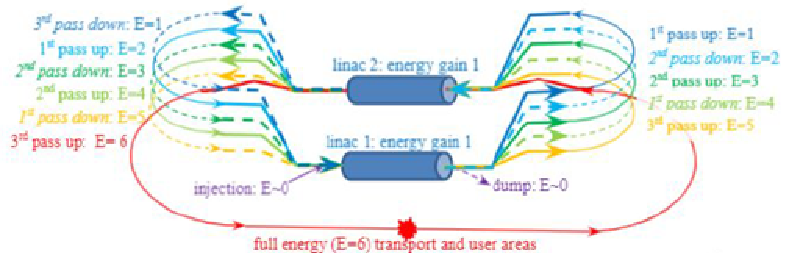
\includegraphics[width=0.8\textwidth]{Figures/DIANA_Inverse_Compton_Source_Design/DIANA_diagram_placeholder.pdf}
\caption{Drawing of the 3-turn DIANA ERL, utilising dual symmetric linacs and separate transport -- where each accelerating and decelerating pass is transported in a separate beamline. A total of 6 different energies will be transported by the DIANA ERL.}
\label{fig:DIANA_ERL_diagram}
\end{figure}
Within the context of the wider accelerator community, DIANA would be a national scale facility and is aligned to two projects in particular: a proposal for the UK-XFEL \cite{burnett2020uk} and as a solution for the Large Hadron--electron Collider (LHeC) \cite{valloni2013strawman,bruning2019exploring,holzer2021accelerator,agostini2021large}. Within the wealth of accelerator solutions to a UK x-ray free electron laser presented in the UK-XFEL science case \cite{burnett2020uk}, a partial ERL solution with an ICS source is suggested. The UK-XFEL ICS source design is a precursor to the DIANA ICS source design, as DIANA could be a potential demonstrator for the UK-XFEL project. The DIANA ERL could also act as a proof-of-principle for the LHeC ERL alongside the existing PERLE accelerator \cite{angal2018perle}, demonstrating another design and transport approach.

High brilliance electron beams on the \si{\giga\electronvolt}-scale can facilitate applications such as a high-power extreme ultraviolet (EUV) FEL and a $\gamma$-ray inverse Compton scattering source. Tunability of the electron bunch energy of the ERL is necessary for many light source experiments and must be central to the design philosophy of DIANA for useful operation of the ICS source and EUV FEL. An EUV FEL source would have far-reaching consequences for semiconductor lithography providing an unparalleled source of 13.5~\si{\nano\meter} EUV radiation (or some harmonic thereof) \cite{socol2011compact}. Whereas a high flux, narrowband $\gamma$-ray inverse Compton scattering source driven by an ERL would have considerable impact upon nuclear physics and security \cite{budker2021expanding}, beyond the bandwidth limited achievements and opportunities available at storage ring facilities such as HI$\gamma$S \cite{weller2009research}. Within the scope of this thesis, the focus is on the development of the latter application as well a progress toward a conceptual design of the DIANA ERL. Hence, the following chapter excludes EUV FEL developments.

The DIANA ICS source will be driven by the ERL electron bunch with interaction points designed directly into the transport optics, unlike the bypass design for the CBETA ICS in Chapter~\ref{CBETA_Inverse_Compton_Scattering_Source_Design}, to produce a multi-colour $\gamma$-ray source taking advantage of the three nominal electron bunch energies of the DIANA ERL (resulting from the three turns). A high average power 4-mirror Fabry-Perot optical re-circulation cavity is proposed to store the laser pulse and interact the laser pulses with the electron bunches at a high repetition rate, producing a high flux and making use of the re-circulated nature of an electron bunch in an ERL; a schematic of the ICS interaction is shown in Fig.~\ref{fig:DIANA_interaction}}. A variable aperture circular collimator placed 10~\si{\meter} from the interaction point will then select the user-desired portion of the spectral output for narrowband operation, taking advantage of the energy--angle correspondence. Through an outline of the ERL, with a focus toward $\gamma$-ray production, and design of the interaction points using optimisation procedures developed in Chapter~\ref{Optimisation_and_Characterisation_of_Inverse_Compton Scattering_Spectra}, the DIANA ICS source aims to produce narrowband ($< 1$\% \textit{rms} BW) radiation on the \si{\mega\electronvolt}-scale. 
\begin{figure}[!h]
\centering
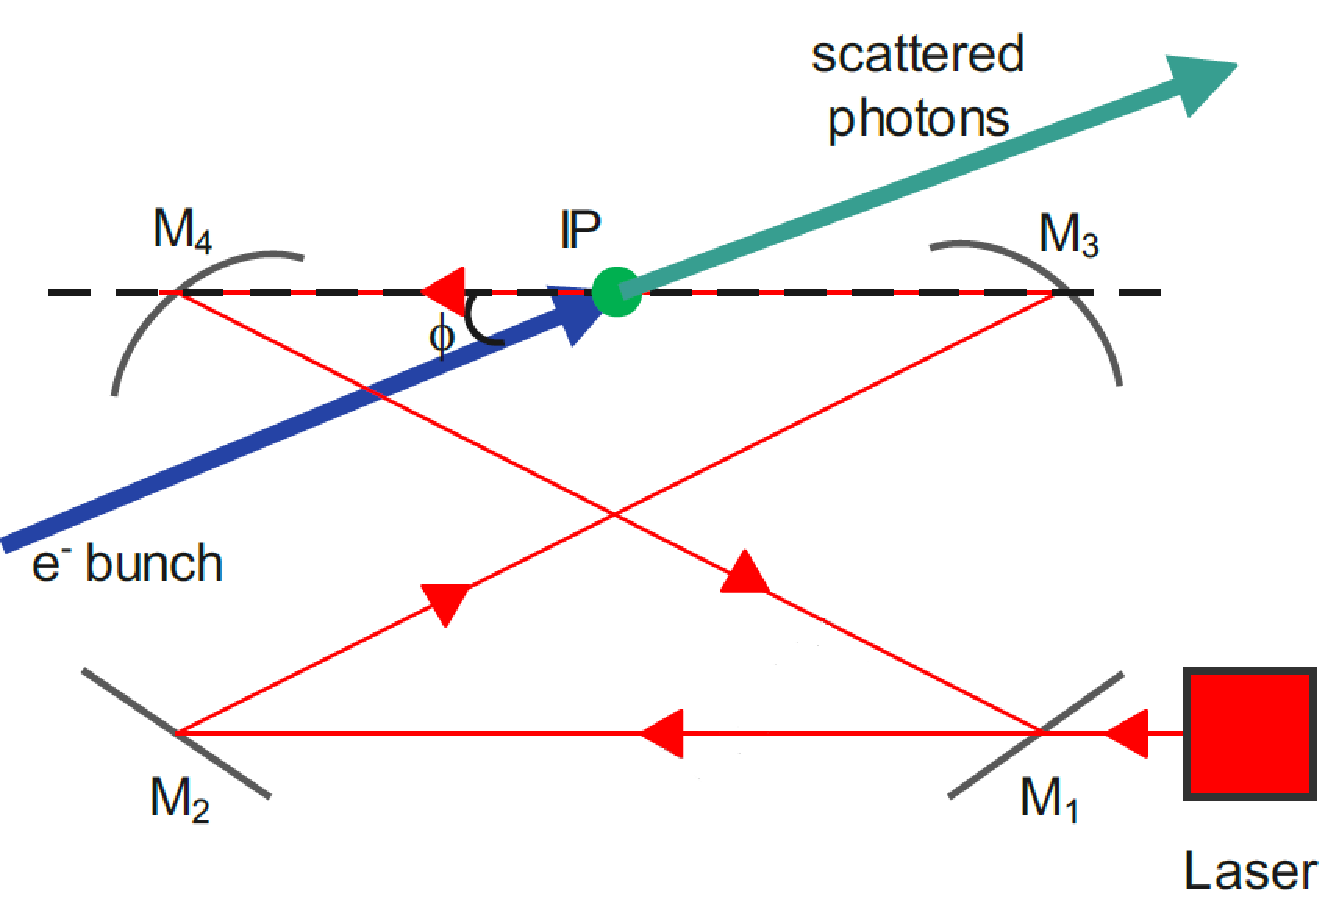
\includegraphics[width=0.6\textwidth]{Figures/DIANA_Inverse_Compton_Source_Design/DIANA_interaction_fixed.pdf}
\caption{}
\label{fig:DIANA_interaction}
\end{figure}

A $\gamma$-ray ICS source at moderate energies ($E_{\gamma} < 5$~\si{\mega\electronvolt}) could enable applications such as nuclear resonance fluorescence (NRF) for inspection of nuclear fuel rods, waste studies and detection of clandestine nuclear material \cite{angell2015demonstration,bolind2015states} whereas higher energy allows ($E_{\gamma} > 5$~\si{\mega\electronvolt}) applications such as nuclear photonics \cite{budker2021expanding} and medical isotope production \cite{habs2011production}. The scattered photon energy regime of nuclear photonics lays in the $\sim$20~\si{\mega\electronvolt} regime and above -- limited in energy by the electron bunch energy of the DIANA ERL. However, the scattered photon energy of the DIANA ICS can be extended to $\sim$40~\si{\mega\electronvolt} through use of frequency doubled lasers (see Section~\ref{sec:lasers_fabry_perot}) such as the commonly used 2nd harmonic of a Nd:YAG ($\lambda =$532~\si{\nano\meter}) laser. Within the applications of a DIANA ERL driven ICS source, special consideration is given to the photo-nuclear production of medical isotopes. 

\section{DIANA ERL Design}
\label{sec:DIANA_ERL_design}

Design of the DIANA energy recovery linac is an ongoing project and fully fledged design studies for the accelerator are incomplete. A full design study of the DIANA ERL is beyond the scope of this thesis, and many first-glance design choices require further investigation and consideration. However, two of the most critical design choices -- the choice of dual linacs and single transport -- can be expanded upon here, with reference to the development of DIANA as a light source facility with a focus on the proposed multi-colour ICS source. Therefore, the  following sections aim to present a non-comprehensive discussion of the design choices with reference to design of a multi-colour ICS source and in the context of other similar ERL projects: the PERLE ERL \cite{angal2018perle}, the ER@CEBAF multi-turn ERL \cite{meot2016er} and the ERL FEL design by Akkermans et al \cite{akkermans2017compact}. 

\subsection{Dual Linacs}

Currently, dual symmetric SRF linacs are incorporated into the straights of the DIANA ERL racetrack layout. Using dual linacs in this scheme minimises the footprint of the accelerator as compared to a design like the CBETA ERL in Chapter~\ref{CBETA_Multi-Pass_Commissioning}, the required acceleration section can be halved. Energy recovery linacs such a PERLE \cite{angal2018perle} and CEBAF \cite{meot2016er} achieve high energies in a compact layout primarily because of the dual linac racetrack design. However, an extra two spreader sections are required to recombine the 3 turns (6 passes) of DIANA into a single beamline for on-axis traversal of the second linac then splitting the beamline into the 6 different passes. Using symmetric linacs (see Section~\ref{sec:dual_linac_ERL}) would mean that the energies transported in the beamlines are spaced by equal successive intervals -- with an energy gain per turn of 355~\si{\mega\electronvolt}, the beamlines after each linac pass vary by 177.5~\si{\mega\electronvolt}. The energy symmetry of passes may mean that spreader design is more simplistic however, an asymmetric solution may be easier to implement. In addition, with 6 passes, as would be necessary with separate transport (see Section~\ref{sec:ERL_transport_options}), the spreader sections would be spatially complex with many nearby magnets experiencing cross-talk -- where magnetic fields overlap -- which would be difficult to design and implement. Multi-turn single transport spreaders have not been demonstrated with a dual linac approach, as both CEBAF \cite{meot2016er} and PERLE \cite{angal2018perle} are common transport ERLs. 

Dual symmetric linacs mean a total of 6 different electron energies would be present in the DIANA ERL i.e each turn contains two electron energies. The additional electron energies are available to a potential light source operating on the ERL, therefore this could provide a simple route to a multi-colour $\gamma$-ray source if an ICS source interaction point is placed after each linac pass. Fully integrated interaction points within the DIANA design would avoid the necessity of complex bypass designs like those for the CBETA ICS source in Section~\ref{sec:bypass_design}. However, with more electron energies transported in the ERL the transport optics must be designed to transport a wider variety of energies. To the authors knowledge, dual linac multi-turn ERLs have not been proposed for light source operations but may provide a useful, tuneable source of electrons at a variety of energies within a compact footprint.

\subsection{Single Transport}

The single transport approach to multi-turn ERLs -- where each accelerating and decelerating configuration of the electron bunch, at each nominal electron energy is transported in a separate beamline (see Section~\ref{sec:ERL_transport_options}) -- has been utilised previously in the ERL FEL design by Akkermans et al \cite{akkermans2017compact}. Therefore, single transport is a more established option for ERL based light sources, such as the DIANA proposal, than common transport approaches which have not demonstrated light source operation. Single transport may be particularly useful for ERL driven ICS source development as each beamline transports a single electron bunch configuration (accelerating or decelerating) at a single energy and therefore varying the optics of a single beamline does not vary optics of other beamlines as long as the electron bunch at the entrance to the linac for the next pass remains unchanged. Therefore, interaction points with variable focusing -- as needed to provide narrowband optimised radiation production (see Chapter~\ref{Optimisation_and_Characterisation_of_Inverse_Compton Scattering_Spectra}) -- can easily be integrated into this design.

In comparison, for a common transport ERL an ICS interaction point would have to focus both electron bunches on the accelerating and decelerating passes to the same electron bunch spot size at the interaction point and, as the produced spectrum of scattered photons is sensitive to the electron bunch distribution, the bunch would have to be in an identical configuration or the ICS spectral output to a user would be variable. Single transport is consequently a more simple transport option for a multi-turn ERL light source. However, single transport ERLs typically use more magnets and beamline infrastructure which adds to the expense of an ERL project. In addition, the aforementioned spreader problem -- due to complexity of multiple electron beams of varying energy traversing the same linac -- are exacerbated by single transport as more beamlines have to be directed through the linac.  

\section{ERL ICS Electron Beam and Optical Cavity Laser Pulse Parameters}

\subsection{ERL ICS Electron Beam Parameters }
\label{sec:DIANA_electron_parameters}

The proposed electron bunch parameters for the DIANA ERL ICS source are presented in Table~\ref{tab:DIANA_electron_beam_design_parameters}. The DIANA electron bunch parameters target a high brilliance (small emittance, high bunch charge) electron bunch for operation of a high quality ICS and FEL light source facility. The electron bunch parameter set focuses on maximising the output of a narrowband ICS source, however the proposed parameters are broadly applicable to development of a high brilliance FEL, where some adjustment to the longitudinal parameters would be neccesary for an FEL due to coherence in FELs requiring short bunch lengths and high peak powers.    
Baseline electron bunch parameters are proposed to characterise the bare, uncollimated spectrum of the produced radiation from the DIANA ICS source where the ICS source is configured solely for high flux operation, not for narrow bandwidth. High flux operation of an ICS $\gamma$-ray source requires small electron bunch spot sizes, therefore a small $\beta$-function at the IP in the baseline case is specified ($\beta^{*}=0.2$~\si{\meter}). Round beams at the IP for the baseline case are specified for simplicity, and because a round bunch is a decent approximation to electron bunches in ERLs. Constant $\beta$-functions in the baseline case allow the effect of varying electron bunch energy in each turn to be inspected. Radiation production is quantified by performance parameters such as the uncollimated flux (Eq.~\ref{eq:flux_angular_crossing_hourglass}), spectral density (Eq.~\ref{eq:spectral_density}), average (Eq.~\ref{eq:average_brilliance}) and peak (Eq.~\ref{eq:peak_brilliance}) brilliance, as calculated in Table~\ref{tab:DIANA_spectral_output} for the DIANA ICS, which can be satisfactorily calculated for an uncollimated ICS source and as such are limited to the baseline case here. Because ICS sources, and light sources more generally, are compared via these performance parameters the baseline case enables comparison between the proposed DIANA ICS source design and other projects, as shown in Section~\ref{sec:gamma_ICS_comparison}, which may not be designed toward the narrowband radiation production goals of DIANA.

The electron bunch parameters have also been optimised for narrowband operation ($\left(\Delta E_{\gamma}<1\%\right)$) of the ICS source using the simplex non-round beam optimisation in Section~\ref{sec:NRB_optimisation}, as this optimisation produced the highest collimated flux within the specified bandwidth for the source. Narrowband optimisation provides insight on the ability of the ICS source design to provide quasi-monochromatic radiation that is most useful to users and for high precision nuclear physics experiments. Single point optimisations are specified for a 0.5\% \textit{rms} bandwidth, chosen because this is conveniently in the centre of the narrowband range and also is comparable to the design bandwidth ($\Delta E_{\gamma}/E_{\gamma}=0.5\%$ FWHM) for the ELI-NP-GBS flagship $\gamma$-ray ICS source \cite{elinp2019vega}. Tuning curve optimisations shown later in this section (in Figs.~\ref{fig:DIANA362_param}, \ref{fig:DIANA717_param}, \ref{fig:DIANA1072_param}), with solution space results in Section~\ref{sec:DIANA_spectral_output}, are performed across the narrowband range (0--1\% \textit{rms} bandwidth).    

\begin{table}[!h]
\centering
\caption{Electron beam parameters foreseen at the DIANA ICS source interaction point (IP). Baseline parameters assume a round transverse profile for the electron bunch whereas the optimised parameters are the result of simplex non-round beam optimisation. The given baseline parameters -- which assume the same $\beta^*$ at the IP -- allow a comparison of flux and bandwidth at different energies. The optimised values beneath those are designed to maximise the flux into a 0.5\% \textit{rms} scattered photon bandwidth through a trade-off of $\beta$-function of the electron bunch in each transverse plane and collimation angle.}
\vspace{3mm}
\begin{threeparttable}
\resizebox{\columnwidth}{!}{
\begin{tabular}{lccccc}
\hline\hline
Parameter & \multicolumn{3}{c}{Quantity} & Unit \\
\hline
Turn number & 1 & 2 & 3  \\
Injection Energy, $E_{\mathrm{inj}}$ & \multicolumn{3}{c}{7} & \si{\mega\electronvolt}\\
\tnote{$\dagger$}~Electron kinetic energy, $E_e$ & 362 & 717 & 1072 & \si{\mega\electronvolt}\\
Harmonic Frequency, $f$ & \multicolumn{3}{c}{125} & \si{\mega\hertz}\\
Bunch charge, $e N_e$ & \multicolumn{3}{c}{100} & \si{\pico\coulomb} \\
Avg. beam current, $I$ & \multicolumn{3}{c}{12.5} & \si{\milli\ampere} \\
Transverse normalised \textit{rms} emittance, $\epsilon_{N}$ & \multicolumn{3}{c}{0.5} & \si{\milli\meter}-\si{\milli\radian}\\
\tnote{$\sharp$}~\textit{rms} bunch length, $\Delta \tau$ & \multicolumn{3}{c}{0.9 (3)} & \si{\milli\meter} (\si{\pico\second})\\
Bunch spacing, $t_{b}$ & \multicolumn{3}{c}{8} & \si{\nano\second} \\
RF frequency, $f_{RF}$ & \multicolumn{3}{c}{750} & \si{\mega\hertz} \\
\tnote{*}~Absolute energy spread, $\Delta E_{e}$ & \multicolumn{3}{c}{$\sim$10--50} & \si{\kilo\electronvolt} \\ 
\tnote{*}~Relative energy spread, $\left(\Delta E_{e}/E_{e}\right)$ & \multicolumn{3}{c}{$\sim5\times 10^{-5}$} & \\
\hline
\multicolumn{5}{c}{Baseline Parameters} \\
\hline
$\beta$-functions at the IP, $\beta_{x}^{*}$/$\beta_{y}^{*}$ & 0.2/0.2 & 0.2/0.2 & 0.2/0.2 & \si{\meter} \\
Electron bunch spot size, $\sigma_{e,x}$/$\sigma_{e,y}$ & 11.87/11.87 & 8.44/8.44 & 6.90/6.90 & \si{\micro\meter}\\
\hline\multicolumn{5}{c}{Optimised 0.5\% \textit{rms} Bandwidth} \\
\hline
$\beta$-functions at the IP $\beta_{x}^{*}$/$\beta_{y}^{*}$ & 1.33/0.298 & 2.62/0.587 & 3.90/0.874 & \si{\meter} \\
Electron bunch spot size, $\sigma_{e,x}$/$\sigma_{e,y}$ & 30.62/14.49 & 30.54/14.46 & 30.48/14.43 & \si{\micro\meter}\\
Collimation Angle, $\theta_{\mathrm{col}}$ & 0.180 & 0.091 & 0.061 & \si{\milli\radian} \\ 
\hline\hline
\end{tabular}}
\begin{tablenotes}
\item[$\sharp$]{Based on the ASML FEL parameters \cite{akkermans2017compact}}
\item[*]{Estimated values.}
\item[$\dagger$]{Electron beam energies to accomplish $E_{\gamma}^{\mathrm{max}}$ = 20~\si{\mega\electronvolt} $\gamma$-rays. $\Delta E_{\mathrm{turn}}$ = 355~\si{\mega\electronvolt}.}
\end{tablenotes}
\end{threeparttable}
\label{tab:DIANA_electron_beam_design_parameters}
\end{table}

% electron bunch energy
The nominal electron kinetic energies of the DIANA 3-turn ERL are 362, 717, 1072~\si{\mega\electronvolt} with a variation in energy per turn of 355~\si{\mega\electronvolt} due to acceleration in the dual linacs with injection of the electron bunch at 7~\si{\mega\electronvolt}. A 7~\si{\mega\electronvolt} injection energy, identical to the PERLE \cite{angal2018perle} ERL injection energy and similar to demonstrated multi-turn ERL projects such as CBETA ($E_{\mathrm{inj}}=6$~\si{\mega\electronvolt}) \cite{bartnik2020cbeta} and S-DALINAC ($E_{\mathrm{inj}}=7.6$~\si{\mega\electronvolt}) \cite{arnold2018first}. \si{\mega\electronvolt}-scale injection energies are relativistic, and above transition, simplifying the dynamics within an ERL (see Chapter~\ref{Energy_Recovery_Linac_Design}). Modern photo-injectors also operate at high current within this energy range, such as the world-leading Cornell photoinjector \cite{bartnik2015operational}. A maximum electron energy of 1072~\si{\mega\electronvolt} is selected as, with a Nd:YAG laser ($\lambda=1064$~\si{\nano\meter}), this allows production of 20~\si{\mega\electronvolt} $\gamma$-rays via inverse Compton scattering necessary for nuclear photonics experiments\cite{budker2021expanding} at the frontier of nuclear physics. The 1072~\si{\mega\electronvolt} maximum energy also reflects the limitations imposed upon the ERL by both physical size and coherent synchrotron radiation losses. For example, assuming a 20~\si{\mega\volt}/\si{\meter} accelerating electric field \cite{ben2006review}, symmetric linacs and an 80\% filling factor (assumed from CBETA \cite{hoffstaetter2017cbeta}) the length of the linacs would be required to be $\sim$11~\si{\meter}, and the accelerator would be expected to have a $\sim$100's~\si{\meter} circumference. Because of the maximum electron energy requirements, the nominal energies of the previous turns are fixed at 362~\si{\mega\electronvolt} and 717~\si{\mega\electronvolt}, with a 355~\si{\mega\electronvolt} energy gain per turn. However, the first turn electron energy is particularly advantageous, as this is proposed to produce scattered photon energies within the energy range for nuclear resonance fluorescence experiments \cite{angell2015demonstration,quiter2011transmission}.          
% RF Frequency + electron bunch frequency
An RF frequency of 750~\si{\mega\hertz} for the DIANA superconducting RF linacs is proposed, as studies for the LHeC ERL configuration have proposed similar RF frequencies ($f_{\mathhrm{RF}}=802.5$~\si{\mega\hertz}) \cite{agostini2021large}, because this is typical of state-of-the-art SRF developments within SRF technologies where stable CW acceleration is available in the 600--800~\si{\mega\hertz} range \cite{calaga2013proposal}. For example, a Jefferson Laboratory prototype single cell SRF cavity has achieved accelerating gradient of $E_{\mathrm{acc}}=25$~\si{\mega\volt}/\si{\meter} at a 748.5~\si{\mega\hertz} RF frequency \cite{rimmer2007jlab}, which would satisfy the DIANA ERL design parameters. 

The proposed bunch repetition frequency of DIANA is 125~\si{\mega\hertz}, 1/6th of the RF frequency of the linac at 750~\si{\mega\hertz}, as DIANA is a 3 turn ERL with both accelerating and decelerating bunches. The electron bunch repetition rate is bound since the laser pulse and electron bunch must interact at the same rate, therefore the Fabry-Perot optical cavity must have an identical repetition frequency (or some harmonic thereof) for interaction of each electron bunch with a laser pulse. The ideal repetition frequency of both systems is 125~\si{\mega\hertz} because of the laser pulse optical re-circulation cavity limitations mentioned in Section~\ref{sec:DIANA_laser_fabry_perot}.

% Beam Current (Bunch Charge and REP FREQ dependence) + emittance
Average current of the electron bunch in DIANA is 12.5~\si{\milli\ampere}, which is dependent upon the bunch charge and the bunch repetition frequency. The electron bunch repetition frequency is limited to 125~\si{\mega\hertz} by the repetition rate of the laser pulse in the optical cavity, and the proposed bunch charge is 100~\si{\pico\coulomb}. Modern photo-injectors are capable of delivering bunch charges into the 100's~\si{\pico\coulomb} range \cite{angal2018perle,hounsell2021optimization} -- for example the Cornell photoinjector demonstrated a 100~\si{\pico\coulomb} electron bunch with a transverse emittance of $\epsilon_{nx} \left(\epsilon_{ny}\right) = 0.37 (0.39)$~\si{\milli\meter}--\si{\milli\radian} \cite{bartnik2015operational}. Therefore, the small transverse emittance proposed for the DIANA ERL ($\epsilon_{n}=0.5$~\si{\milli\meter}--\si{\milli\radian}) is also well within the state-of-the-art.

Transport of the DIANA bunch charge and small normalised emittance is supported by a previous design study for an EUV FEL using a multi-turn ERL with a 100~\si{\pico\coulomb} bunch charge and similar transverse normalised emittance \cite{akkermans2017compact}. ERLs have been operated on the 10's~\si{\pico\coulomb}-scale, such as the J-Lab FEL, which demonstrated energy recovery with 60~\si{\pico\coulomb} electron bunches \cite{benson1999first}. The average power of the DIANA electron beam is 13.4~\si{\mega\watt}, a factor of 2.23 larger than the electron beam power in the CBETA ERL proposal as described in Chapter~\ref{CBETA_Multi-Pass_Commissioning}, and similar to the PERLE proposal \cite{angal2018perle}. However, average current is fundamentally limited by collective effects such as CSR and beam break-up instabilities arising during transport in the ERL, as in CBETA, so more in depth studies -- beyond the scope of this thesis -- are required to validate the proposed parameters. 

% Bunch length
Short \textit{rms} bunch lengths (durations) of $\sigma_{z}=0.9$~\si{\milli\meter} (3~\si{\pico\second}), \textit{rms}), based upon the bunch length in the ASML associated ERL-FEL \cite{akkermans2017compact}, are proposed for the DIANA ERL. However, a short electron bunch duration is only desirable for an ICS source interaction if the time duration of the radiation is critical for applications because the electron bunch duration is proportional to the duration of the scattered radiation, unlike in FEL operation where a short bunch length is required for coherence and a high peak beam current. The scattered photon duration of ICS sources is also subject to the laser pulse duration, so no benefit is found for electron bunch lengths much shorter than the laser pulse duration in the Fabry-Perot optical cavity. The 3~\si{\pico\second} electron bunch duration is similar to the 10's~\si{\pico\second} pulse durations demonstrated in Fabry-Perot optical cavities. A 3~\si{\pico\second} bunch duration also ensures minimal luminosity reduction from the angular crossing of the ICS interaction and the hourglass effect of the two diverging beams, as seen via inspection of (Eq.~\ref{eq:miyahara_combined_reduction}). 

% Bunch Energy Spread
A small electron bunch energy spread is necessary for the production of narrowband radiation from both an ICS source and a FEL. The bandwidth of an ICS source is directly proportional to the energy spread of the of the electron bunch (Eq.~\ref{eq:RMS_bandwidth}), therefore it is necessary to minimise the energy spread of the electron bunch for light source operations. The electron bunch energy spread proposed for DIANA in Table~\ref{tab:DIANA_electron_beam_design_parameters} ($\Delta E_{e} \sim 10$~\si{\kilo\electronvolt}) is based upon the 6~\si{\kilo\electornvolt} uncorrelated electron energy spread that is readily demonstrated at the EuXFEL \cite{tomin2021accurate} for a 250~\si{\pico\coulomb} electron bunch. 

% Optimisations
The three DIANA ICS sources have been optimised for a 0.5\% \textit{rms} bandwidth using the three optimisation methods (RB, simplex NRB and GA NRB) outlined in Chapter~\ref{Optimisation_and_Characterisation_of_Inverse_Compton Scattering_Spectra}. The optimised electron beam interaction parameters and collimation parameters resulting from the single point 0.5\% \textit{rms} bandwidth optimisations are shown in Table~\ref{tab:DIANA_electron_beam_design_parameters}. However, the focus here is on the tuning curve optimations in the narrowband range ($0 \leq \Delta E_{\gamma}/E_{\gamma} \leq 1$\% \textit{rms} bandwidth). Laser pulse parameters remain unchanged from Table~\ref{tab:DIANA_laser_pulse_design_parameters}. Tuning curves are produced for each of the three nominal electron energies of the DIANA ERL (362, 717, 1072~\si{\mega\electronvolt}).

\begin{figure}[!h]
\centering
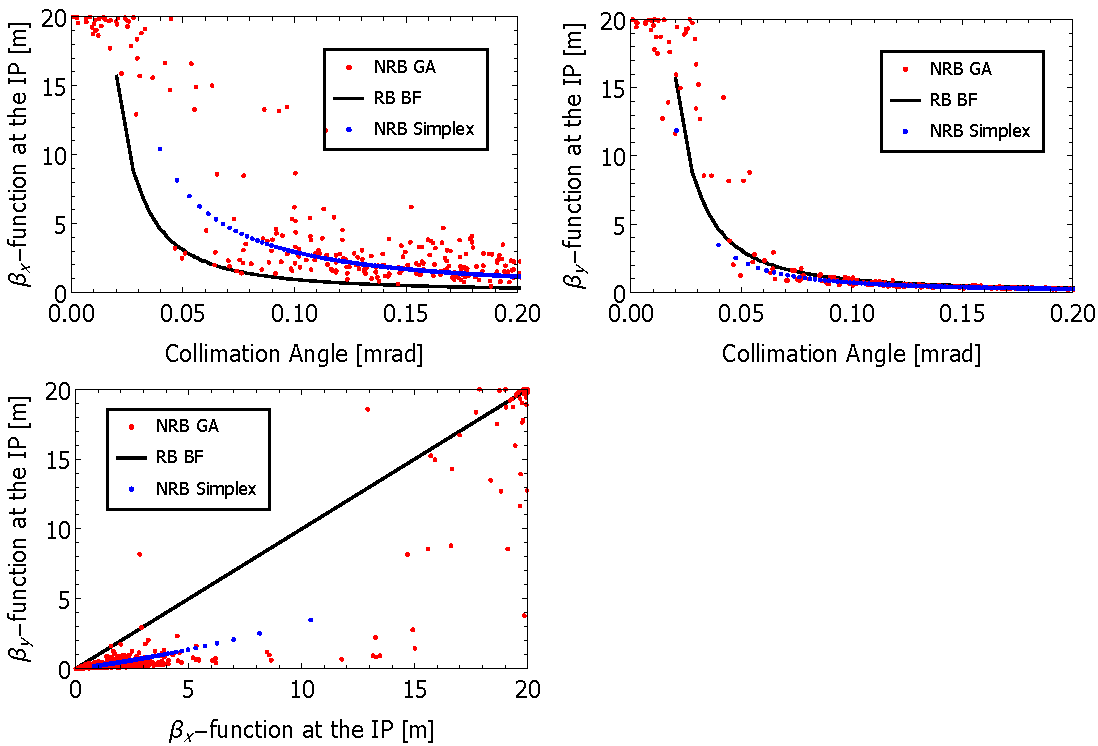
\includegraphics[width=\textwidth]{Figures/DIANA_Inverse_Compton_Source_Design/DIANA362param.pdf}
\caption{DIANA 362~\si{\mega\electronvolt} 1st turn ICS source optimisations, comparing the two non-round beam approaches (simplex (blue) and GA (red)) and the round beam approach (black). Top Left: parameter space of the interaction $\beta$-function in the $x$ plane and collimation angle for optimised cases. Top Right: parameter space of the interaction $\beta$-function in the $y$ plane and collimation angle for optimised cases.  Bottom Left: interaction point $\beta$-function parameter space in the $x$ and $y$ plane for optimised cases. }
\label{fig:DIANA362_param}
\end{figure}

The top plots in Fig~\ref{fig:DIANA362_param} show the $\beta$-functions at the IP in each plane against the required collimation angle for each of the three optimisation methods under consideration. The $\beta_{x}^{*}$--$\theta_{\mathrm{col}}$ plot shows that the non-round beam optimisations maintain the `elbow' shape as evident in the non-round beam case, however the simplex optimisation is offset from the round beam solution and the gradient of the `elbow' shape is less severe. The small collimation angle (large $\beta$-function) end of the `elbow' typically relates to the narrowest bandwidth portion of the tuning curve whereas the large collimation angle (small $\beta$-function) solutions relate to larger bandwidths in the range; maximising collimation angle and minimising $\beta$-functions in each plane is optimal for collimated flux (Eq.~\ref{eq:collimated_flux}) but these solutions are bound by the bandwidth (Eq.~\ref{eq:RMS_bandwidth}). The genetic algorithm $\beta_{x}^{*}$--$\theta_{\mathrm{col}}$ parameter space shows a large stratification of optimal configurations in this plot which highlights the weak dependence on both bandwidth and collimated flux of the $\beta_{x}^{*}$ parameter. However, the $\beta_{y}^{*}$--$\theta_{\mathrm{col}}$ plot shows less stratification for the $\beta_{y}^{*}$ parameter and this also adheres closer to the round beam solution for both the genetic algorithm and simplex cases. Therefore, we can conclude that the variation of the non-round beam in comparison to the round beam case observed in the electron bunch transverse size $x$-plane must be due to the angular crossing, which is the only difference between the two planes.

Plots of the selected $\beta$-functions at the IP in each plane parameter space points corresponding to the Pareto front points in the collimated flux--\textit{rms} bandwidth space in Fig~\ref{fig:DIANA362_param} show that, as the transverse emittance is identical in each plane, the solution in the simplex and GA optimisations for the IP configuration is to have a larger electron bunch spot size in the $x$-plane than the $y$-plane, as the $\beta_{x}$ functions are larger than the $\beta_{y}$ functions. Solutions for the $\beta$-functions in each plane clearly diverge from the linear relationship (shown for the round beam case), therefore the use of NRB optimisations is justified. However, the genetic algorithm points are clearly quite polarised to a pair of high $\beta$-functions in each plane or low $\beta$-functions in each plane; the high $\beta$-function solutions correspond to the narrowest bandwidth solutions.

\begin{figure}[!h]
\centering
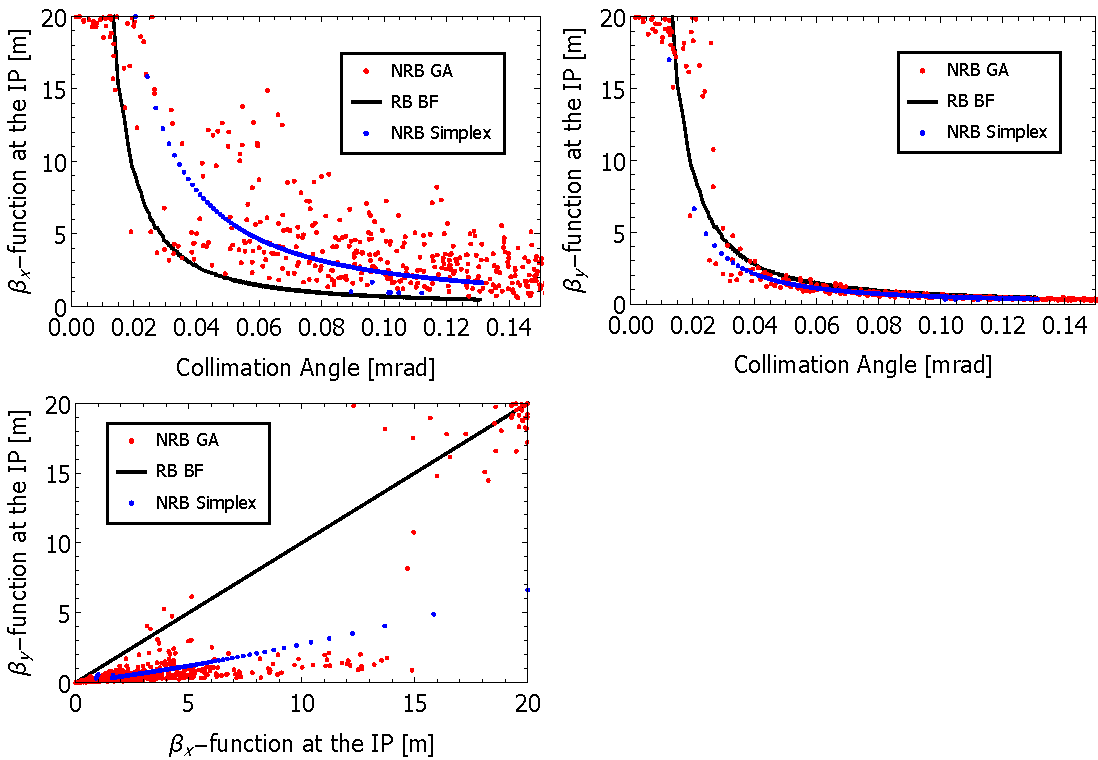
\includegraphics[width=\textwidth]{Figures/DIANA_Inverse_Compton_Source_Design/DIANA717param.pdf}
\caption{DIANA 717~\si{\mega\electronvolt} 2nd turn ICS source optimisations, comparing the two non-round beam approaches (simplex (blue) and GA (red)) and the round beam approach (black). Top Left: parameter space of the interaction $\beta$-function in the $x$ plane and collimation angle for optimised cases. Top Right: parameter space of the interaction $\beta$-function in the $y$ plane and collimation angle for optimised cases. Bottom Left: interaction point $\beta$-function parameter space in the $x$ and $y$ plane for optimised cases. }
\label{fig:DIANA717_param}
\end{figure}

The 717~\si{\mega\electronvolt} parameter space tuning curves in Fig.~\ref{fig:DIANA717_param} shows similar properties to the parameter space of the 362~\si{\mega\electronvolt} tuning curve in Fig.~\ref{fig:DIANA362_param}. However, the collimation angles in this case are smaller because of the acceptance angle dependence on energy ($\Psi=\gamm\theta$). A non round beam solution is still achieved by both the simplex and GA NRB optimisations, as the GA and simplex solutions in the bottom left plot in Fig.~\ref{fig:DIANA717_param} vary from the RB solution. Again, larger horizontal $\beta$-functions are favoured ($\beta_{x}>\beta_{y}$) which means the transverse profile of the electron bunch is larger horizontally resulting from the crossing angle in the $x$--$z$ plane. The NRB solutions in the $\beta_{y}$--$\theta_{\mathrm{col}}$ plot are more similar to the RB solutions than in the $\beta_{x}$--$\theta_{\mathrm{col}}$ plot, and the GA points are less stratified here.    

\begin{figure}[!h]
\centering
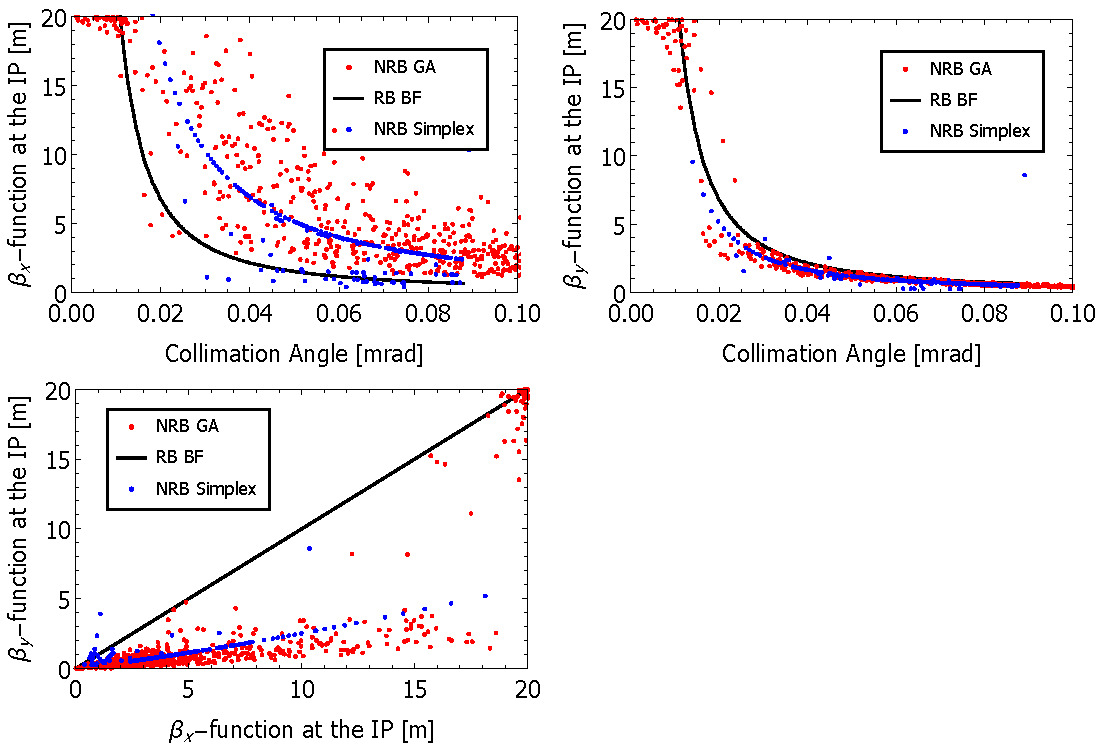
\includegraphics[width=\textwidth]{Figures/DIANA_Inverse_Compton_Source_Design/DIANA1072param.pdf}
\caption{DIANA 1072~\si{\mega\electronvolt} 3rd turn ICS source optimisations, comparing the two non-round beam approaches (simplex (blue) and GA (red)) with the round beam approach (black). Top Left: parameter space of the interaction $\beta$-function in the $x$ plane and collimation angle for optimised cases. Top Right: parameter space of the interaction $\beta$-function in the $y$ plane and collimation angle for optimised cases. Bottom Left: interaction point $\beta$-function parameter space in the $x$ and $y$ plane for optimised cases.}
\label{fig:DIANA1072_param}
\end{figure}

Fig.~\ref{fig:DIANA1072_param} shows the parameter space tuning curves corresponding to the optimal collimated flux--\textit{rms} bandwidth solutions in the range 0--1\% \textit{rms} bandwidth. The `elbow' shapes are again visible in all $\beta_{x/y}$--$\theta_{\mathrm{col}}$ plots however, the collimation angles of the solutions are smaller than the 717~\si{\mega\electronvolt} electron bunch energy case. NRB solutions are again favoured in the $\beta_{x}$--$\beta_{y}$ plot, with $\beta_{x}>\beta_{y}$ resulting in an elliptical electron bunch spot size at the IP. Within the $\beta_x$--$\theta_{\mathrm{col}}$ plot, there are some simplex NRB optimisations points which do not correspond to the overall `elbow' trend, these points appear to be closer to the RB solution and could be points in which the simplex optimisation has become trapped in a local minima. 

Overall, for the parameter space tuning curves in Figs.~\ref{fig:DIANA362_param}, \ref{fig:DIANA717_param}, \ref{fig:DIANA1072_param}, the GA NRB and simplex RB solutions show good agreement. The NRB solutions clearly deviate from the RB solutions in each nominal electron bunch energy case, hence applying a NRB optimisation is advantageous to the DIANA ICS. Collimation angle also appears to vary with energy; smaller collimation angles are favoured at higher energy which is understandable because the opening angle of the produced radiation is related to $1/\gamma$, as explained in Section~\ref{sec:electron_photon_interaction_cross_section}.    

\subsection{Optical Cavity and Laser Pulse Parameters}
\label{sec:DIANA_laser_fabry_perot}

% Why re-circ + Nd:YAG?
A Nd:YAG laser ($\lambda = 1064$~\si{\nano\meter}), re-circulated using a 4 mirror Fabry-Perot optical cavity, with a 5\si{\degree} crossing angle is proposed for the DIANA ICS source, as shown in Fig.~\ref{fig:DIANA_interaction}. A re-circulated laser pulse scheme, where a 10's--100's~\si{\micro\joule} laser pulse is makes many round trips of an optical cavity, is selected to take advantage of the 100's~\si{\mega\hertz} repetition rates available from the DIANA ERL. Explanation of the operation of an ICS source with a Fabry-Perot optical cavity is explained in Section~\ref{sec:lasers_fabry_perot}. As noted in Section~\ref{sec:lasers_fabry_perot}, the average laser power of the re-circulated scheme is larger which is necessary for a high-flux source, whilst the peak properties of the radiation are less critical to the main applications --  nuclear resonance fluorescence and medical isotope production -- of such a source. As in the CBETA ICS source design, the cERL Fabry-Perot cavity \cite{akagi2016narrow} is the basis for the cavity used in the DIANA ICS source and a full design is beyond the scope of this thesis.

% 4-mirror + Nd:YAG selection 
Envisioned parameters of the laser pulse provided by a Nd:YAG ($\lambda = 1064$~\si{\nano\meter}) laser and a four mirror Fabry-Perot optical cavity for use in the DIANA ICS source are shown in Table~\ref{tab:DIANA_laser_pulse_design_parameters}. As noted in Section~\ref{sec:lasers_fabry_perot}, a 4 mirror cavity is selected over a 2 mirror design for improved stability of operation and better focal properties. Following the example of the CBETA ICS source (Chapter~\ref{CBETA_Inverse_Compton_Scattering_Source_Design}), an Nd:YAG laser is selected for its relatively short pulse duration ($\tau_{\mathrm{laser}}=10$~\si{\pico\second}), narrow spectral bandwidth and because the incident photon energy ($E_{L}=1.17$~\si{\electronvolt}) is sufficient to produce 20~\si{\mega\electronvolt} $\gamma$-rays from \si{\giga\electronvolt}-scale electron bunches. 

\begin{table}[!h]
\centering
\caption{Nd:YAG Gaussian laser pulse parameters at the CBETA ICS IP. The interacted laser pulse is produced via a Nd:YAG infrared laser and re-circulated in a bow-tie Fabry-Perot optical cavity.}
\begin{tabular}{lcc}
\hline\hline
Parameter & Quantity & Unit \\
\hline
Wavelength, $\lambda_\textrm{laser}$ & 1064 & \si{\nano\meter}\\
Photon energy, $E_\textrm{laser}$ & 1.17 & \si{\electronvolt}\\
Pulse energy, $E_{pulse}$  & 100 & \si{\micro\joule}\\
Number of photons, $N_{\textrm{laser}}$ & 5.34$\times 10^{14}$ & \\ 
Repetition rate, $f$ & 125 & \si{\mega\hertz}\\
Spot size at the IP, $\sigma_\textrm{laser}$ & 25 & \si{\micro\meter}\\
Crossing angle, $\phi$ & 5 & deg \\
Pulse length, $\tau_{\mathrm{laser}}$  & 10 & \si{\pico\second}\\
Spectral bandwidth (\textit{rms}), $\Delta E_\textrm{laser}/E_\textrm{laser}$ & $6.57\times 10^{-4}$ &   \\
\hline\hline
\end{tabular}
\label{tab:DIANA_laser_pulse_design_parameters}
\end{table}

% Justification of crossing angle
A crossing angle of 5\si{\degree} is imposed in order to prevent the scattered $\gamma$-rays and the electron bunches from impinging on cavity mirrors. Whilst head-on interactions are possible using strong bending interaction regions that can introduce to the IP and remove the electron bunch within the mirror spacing, as is the case in MuCLS \cite{eggl2016munich}, or via mirrors with holes, which reduces gain in optical re-circulation cavities, these may not be advantageously implemented within ERLs. A crossing angle within a 2--12\si{\degree} range is reasonable, whilst being tolerable for integration of cavity components \cite{variola2011luminosity}. A 5\si{\degree} crossing angle is also proposed because this mirrors the demonstrated cERL ICS \cite{akagi2016narrow} Fabry-Perot optical cavity. 

% Justification of rep freq
A repetition frequency of 125~\si{\mega\hertz} results in a cavity path length of 2.4~\si{\meter}, which is tolerable for misalignment errors \cite{zomer2009polarization}, and within the same scale as the 9.2~\si{\meter} MuCLS optical re-circulation cavity \cite{eggl2016munich}. The minimum path length limitation of a Fabry-Perot optical cavity is due to mirror heating, which results in thermoelastic deformation of the optical cavity mirrors causing a loss of stability of the optical cavity \cite{chaikovska2016high}. A further discussion of repetition rate considerations is included in Section~\ref{sec:lasers_fabry_perot}.   

% Justification of Spot size
A \textit{rms} spot size (radius) on the order of 10's~\si{\micro\meter} is common within ICS sources \cite{deitrick2017inverse,drebot2019brixs,dupraz2020thomx}, for example the laser pulse spot size achieved at cERL ICS is 20~\si{\micro\meter}/30~\si{\micro\meter} \cite{akagi2016narrow}, which is similar to the parameters proposed for the DIANA ICS source. The waist size of the ICS source is within the state-of-the-art. Smaller waists are difficult to achieve because of astigmatism in mirrors \cite{zomer2009polarization}, and that the laser pulse spot size upon the cavity mirrors increases as the laser spot size decreases because of the Rayleigh range (Eq.~\ref{eq:rayleigh_range}) which causes further spatial limitations and a larger crossing angle.

% Justification of cavity + stored power
These laser pulse parameters are based upon the demonstration of the Fabry-Perot optical cavity in the cERL ICS experiment \cite{akagi2016narrow}. However, they have been modified for a reduced 125~\si{\mega\hertz} repetition rate with an increased pulse energy of 100~\si{\micro\joule}, resulting in an increased average stored power of 12.5~\si{\kilo\watt} recirculated in the optical cavity. Therefore, the stored power of the Fabry-Perot cavity in the DIANA ICS source is increased relative to the proposed  stored laser power for the CBETA ICS source in Table~\ref{tab:CBETA_laser_pulse_design_parameters}, though the increased power remains within the MuCLS demonstration of 70~\si{\kilo\watt} \cite{eggl2016munich}. However, increased stored average power increases the flux of scattered photons produced from an ICS source. The DIANA optical re-circulation cavity also has an average stored laser power a factor of $\sim50\times$ lower than the state-of-the-art 670~\si{\kilo\watt} average stored power demonstrated by Carstens et al \cite{carstens2014megawatt}, therefore the laser pulse energy and repetition rate (average stored laser power) are feasible. 

% Justification of the spectral bandwidth
The wavelength variation of the proposed incident laser pulse, based on examples of Nd:YAG lasers \cite{thorlabs2021ndyag200}, is characteristically small ($\Delta\lambda = 0.7$~\si{\nano\meter, \textit{rms}}) \cite{corner2019} which results is a small spectral bandwidth of $\Delta E_{L}/E_{L} = 6.57\times 10^{-4}$. A small spectral bandwidth is necessary to a narrowband ICS source as the bandwidth of the scattered radiation (Eq.~\ref{eq:RMS_bandwidth}) is dependent upon the spectral bandwidth. Comparatively, other lasers have a larger spectral bandwidth (see Section~\ref{sec:lasers_fabry_perot}) therefore the Nd:YAG laser is practical for development of a narrowband ICS source. 

\section{ICS Source Spectral Output}
\label{sec:DIANA_spectral_output}

The anticipated spectral output of the DIANA ICS source, using the electron bunch and laser pulse parameters specified in Tables~\ref{tab:DIANA_electron_beam_design_parameters},~\ref{tab:DIANA_laser_pulse_design_parameters}, is presented in Table~\ref{tab:DIANA_spectral_output}. The spectral output parameters are shown for both the 0.5\% \textit{rms} bandwidth optimised, using the simplex NRB method in Section~\ref{sec:NRB_optimisation}, and the baseline case for small electron bunch spot size, with constant $\beta$-functions ($\beta_{x/y}=0.2$~\si{\meter}). The average (Eq.~\ref{eq:average_brilliance}) and peak (Eq.~\ref{eq:peak_brilliance}) brilliance, spectral density (Eq.~\ref{eq:spectral_density}) and uncollimated flux (Eq.~\ref{eq:flux_angular_crossing_hourglass}) have been calculated for the baseline case. The collimated flux (Eq.~\ref{eq:collimated_flux}) can only be calculated for the 0.5\% \textit{rms} bandwidth configuration because the baseline case is used to define the full, uncollimated radiation spectrum. All calculation methods are outlined in Chapter~\ref{Photon_Production_by_Inverse_Compton_Scattering}. 
\begin{table}[!h]
\caption{Anticipated photon output for each of the three nominal electron beam energies (at each turn) DIANA, taking into account a 5\si{\degree} crossing angle. The recoil parameter is small $X < 0.02$, even at 1072~\si{\mega\electronvolt} -- the maximum electron beam energy. The collimated flux has been optimised for a 0.5\% \textit{rms} bandwidth using the NRB simplex optimisation (see Section~\ref{sec:NRB_optimisation}) and the baseline case focuses at the IP to $\beta^{*} =0.2$~\si{\meter} for each nominal electron energy.}
\vspace{3mm}
\centering
\begin{threeparttable}
\begin{tabular}{lcccc}
\hline\hline
 & \multicolumn{3}{c}{Electron Kinetic Energy (\si{\mega\electronvolt})} & \\
 \cline{2-4}
 & 362 & 717 & 1072 & \\
\hline
$\gamma$-ray peak energy  & 2.33 & 9.06 & 20.11 & \si{\mega\electronvolt}\\
\hline
 & \multicolumn{3}{c}{Baseline} & \\
\hline
Source size ($x$/$y$)  & 10.72/10.72 & 8.00/8.00 & 6.65/6.65 & \si{\micro\meter} \\
Uncollimated flux  & 5.77$\times 10^{10}$ & 6.02$\times 10^{10}$ & 6.08$\times 10^{10}$ & ph/\si{\second}\\
Spectral density  & 2.48$\times 10^{5}$ & 6.65$\times 10^{4}$ & 3.03$\times 10^{4}$ & ph/\si{\second} \si{\electronvolt}\\
Average brilliance  & 5.64$\times 10^{12}$ & 2.05$\times 10^{13}$ & 4.45$\times 10^{13}$ & ph/\si{\second} \si{\milli\meter}$^{2}$\si{\milli\radian}$^{2}$ 0.1\% bw\\
Peak brilliance\tnote{*}  & 4.44$\times 10^{18}$ & 1.62$\times 10^{19}$ & 3.50$\times 10^{19}$ & ph/\si{\second} \si{\milli\meter}$^{2}$ \si{\milli\radian}$^{2}$ 0.1\% bw\\
\hline
 & \multicolumn{3}{c}{0.5\% \textit{rms} bandwidth} & \\
\hline
Source Size ($x$/$y$) & 19.36/12.54 & 19.35/12.52 & 19.33/12.50 & \si{\micro\meter} \\ 
Collimated flux  & 1.30$\times 10^{9}$ & 1.29$\times 10^{9}$ & 1.29$\times 10^{9}$ & ph/\si{\second} 0.5\% bw \\
\hline\hline
\end{tabular}
\begin{tablenotes}
\item[*]{(Eq.~\ref{eq:peak_brilliance}) is used to calculate the peak brilliance.}
\end{tablenotes}
\end{threeparttable}
\label{tab:DIANA_spectral_output}
\end{table}

% what energies are possible + tunability
Table~\ref{tab:DIANA_spectral_output} shows the DIANA ICS source is capable of producing $\gamma$-rays up to 20.11~\si{\mega\electronvolt}, with the first two turns nominally producing 2.33 and 9.06~\si{\mega\electronvolt} $\gamma$-rays. The crossing angle ($\phi=5\si{\degree}$) of the ICS interaction in DIANA reduces the maximum scattered photon energy from 20.14~\si{\mega\electronvolt} to 20.11~\si{\mega\electronvolt} -- a small $\sim 30$~\si{\kilo\electronvolt} reduction. Depending on the tunability of the electron bunch and through variation of the detection angle (due to the energy--angle correspondence), scattered photon energies $< 20.11$~\si{\mega\electronvolt} may be accessible -- steplessly variable tunablility. Tunable $\gamma$-ray energy production will be a focus for future DIANA design work, this is highly dependent on the transport design for the ERL. 

% Why is flux, spec den, avg brill good 
World-leading uncollimated flux, spectral density and average brilliance are available from the DIANA ICS source due to the interaction of a high brightness electron beam with a re-circulated laser pulse at high repetition rate. For example, the maximum flux of HI$\gamma$S \cite{weller2009research} -- the current highest flux $\gamma$-ray ICS source -- is $5\times 10^{8}$~ph/\si{\second}, a factor of $\sim 120$ smaller than the maximum flux of the DIANA ICS source.  A full comparison of the DIANA ICS source to other designed and operated ICS sources on the \si{\mega\electronvolt}-scale in terms of scattered photon energies and flux is presented in Section~\ref{sec:gamma_ICS_comparison}. 

Flux reduces by 5.1\% from the 1072~\si{\mega\electronvolt} highest electron energy (3rd turn) to the 362~\si{\mega\electronvolt}  nominal electron energy of the 1st turn because of the reduction in the electron bunch spot size with energy, which results in increased flux. The small effect increase in the recoil parameter (Eq.~\ref{eq:X_geometry}) decreases the flux, but this is a much smaller effect. A reduction in average and peak brilliance is observed because this is defined as the flux per unit phase space area and the phase space are is Lorentz contracted causing a $\mathcal{B}\propto \gamma^{2}$ dependence, which is explicitly shown in (Eq.~\ref{eq:average_brilliance_compact}). Spectral density (Eq.~\ref{eq:spectral_density}) deceases with increasing electron beam energy as the spectral density is the flux per unit scattered photon energy and the scattered photon energy (Eq.~\ref{eq:scattered_photon_energy}) is double Doppler shifted, yielding a $\mathcal{S}\propto 1/\gamma^{2}$ dependence.  

The flux, spectral density and (average and peak) brilliance of the DIANA ICS source all account for geometric luminosity reduction, as explained in Section~\ref{sec:geometric_luminosity_reduction}, which arises from the crossing angle imposed on the interaction and the hourglass effect \cite{furman1991hourglass}, where the spot size of the diverging electron bunch and laser pulse varies throughout the interaction. The combined luminosity reduction (Eq.~\ref{eq:miyahara_combined_reduction}) of the angular crossing and hourglass effect $R_{ACHG}=0.094$, as derived by Miyahara \cite{miyahara2008luminosity}, causes a factor of 10.6 reduction in the luminosity of the interaction and therefore to the flux, brilliance and spectral density. However, the hourglass effect contribution to the luminosity reduction is negligible in the DIANA case as the electron bunch length ($\sigma_{ze}=0.9$~\si{\milli\meter}, \textit{rms}) and laser pulse length ($\sigma_{zL}=3.0$~\si{\milli\meter}, \textit{rms}) are short.  

% Why is peak brilliance poor?
Peak brilliance of the DIANA ICS source is reduced in the DIANA ICS source in comparison to other proposed ICS sources \cite{barty2011overview}, which are aiming for $<10^{20}$~ph/\si{\second}~\si{\milli\meter}$^{2}$--\si{\milli\radian}$^{2}$~0.1\% BW,  because the focus of DIANA is producing $\gamma$-rays at a high repetition rate and subsequently high average brilliance. The modest peak power of DIANA is due to the low energy of the interacted laser pulse ($E_{\mathrm{pulse}} = 100$~\si{\micro\joule}) and the moderate picosecond durations of the laser pulse ($\tau_{L}=10$~\si{\pico\second}) and electron bunch ($\tau_{e}=3$~\si{\pico\second}). High peak brilliance ICS sources such as the original ELI-NP-GBS design \cite{adriani2014technical} typically target femtosecond electron bunch and laser pulse lengths with Joule-scale laser pulse energies. 

% Single point Narrowband optimisation 
The three DIANA ICS sources have been optimised for a 0.5\% \textit{rms} bandwidth using the non-round beam simplex optimisation method, described in Chapter~\ref{Optimisation_and_Characterisation_of_Inverse_Compton Scattering_Spectra}, because this optimisation method delivers a higher collimated flux (albeit a small $<1$\% variation from the GA method). A 0.5\% \textit{rms} bandwidth has been selected because this is within the $<1$\% \textit{rms} bandwidth limit designated as narrow bandwidth within this work, and 0.5\% \texit{rms} BW is of the order of the ELI-NP-GBS $\gamma$-ray source \cite{elinp2019vega,tanaka2020current} (0.5\% \textit{FWHM} BW), which is the current flagship narrowband $\gamma$-ray production facility under construction in Europe. The optimised electron beam interaction $\beta$-functions and collimation angles resulting from the 0.5\% \textit{rms} bandwidth optimisation are shown in Table~\ref{tab:DIANA_electron_beam_design_parameters}, the collimated flux is calculated using these parameters.

The DIANA ICS source is expected to deliver a collimated flux of 1.30--1.29$\times 10^{9}$~ph/\si{\second} in a 0.5\% \textit{rms} bandwidth, with variation due to the increase in the recoil parameter with electron bunch energy. As the $\beta$-functions are allowed to vary with electron energy in the optimisations, the increase in flux due to the decreasing electron spot size with electron energy observed in the baseline case in Table~\ref{tab:DIANA_spectral_output} is not observed for the optimised case. The RB optimisation (see Section~\ref{sec:RB_optimisation}) for the 1072~\si{\mega\electronvolt} electron bunch energy yields a collimated flux of $1.24\times 10^{9}$~ph/\si{\second} in comparison to the $1.30\times 10^{9}$~ph/\si{\second} for the NRB simplex optimisation, therefore a gain in flux of 4.62\% is achieved via NRB simplex optimisation -- similar results are achieved for the other nominal electron energies.
Collimation also has another benefit as at a collimator, placed 10~\si{\meter} downstream of the interaction point, the spot size (radius) of the radiation produced in a 0.5\% \textit{rms} bandwidth with the 1072~\si{\mega\electronvolt} electron bunch is 0.61~\si{\milli\meter}, therefore DIANA could produce a pencil beam of $\gamma$-rays for experimental use.

To further characterise narrowband operation of the DIANA ICS sources a series of tuning curves have been devised, based on optimisation methods in Chapter~\ref{Optimisation_and_Characterisation_of_Inverse_Compton Scattering_Spectra}, to show the maximum collimated flux as a function of bandwidth within the narrow bandwidth ($<1$\% \tetxit{rms} BW) regime. For optimisation, the laser pulse parameters remain unchanged from Table~\ref{tab:DIANA_laser_pulse_design_parameters} and only the $\beta$-functions at the IP in each plane and the collimation angle are varied. The solution space Pareto-optimal fronts (tuning curves) of the collimated flux--\textit{rms} bandwidth in the narrowband range ($\Delta E_{\gamma}/E_{\gamma} < 1$\%) are shown in Fig.~\ref{fig:DIANA_FBW}, with the corresponding parameter space fronts shown previously in Figs.~\ref{fig:DIANA362_param}, \ref{fig:DIANA717_param}, \ref{fig:DIANA1072_param} and discussed in Section~\ref{sec:sec:DIANA_electron_parameters}.  

\begin{figure}[!h]
\centering
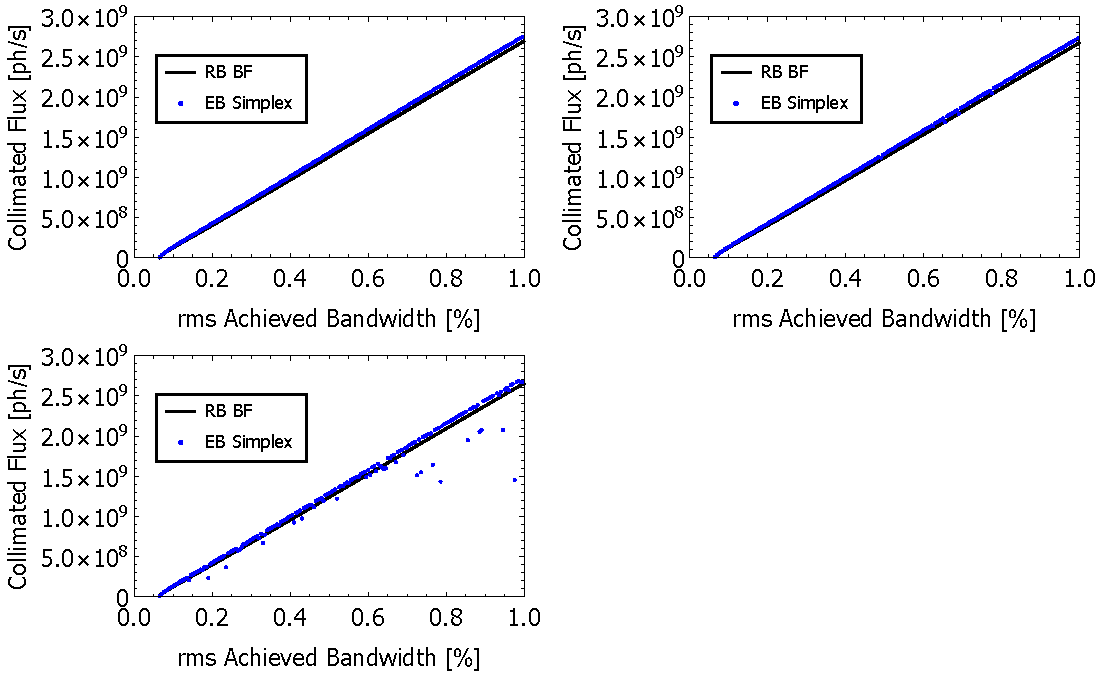
\includegraphics[width=\textwidth]{Figures/DIANA_Inverse_Compton_Source_Design/DIANAFBW.pdf}
\caption{}
\label{fig:DIANA_FBW}
\end{figure}

Fig~\ref{fig:DIANA_FBW} shows the Pareto fronts of the collimated flux--\textit{rms} bandwidth is in good agreement between the simplex and genetic algorithm methods for each of the three nominal electron energies ($E_{e}= $362, 717, 1072~\si{\mega\electronvolt}). A small increase in collimated flux is observed for the NRB optimisations in comparison to the RB optimisations, however the increase is on a percent-scale as a round beam approximation is a good approximation for an ERL due to the small emittance and $\beta$-functions at the IP.

The solution space tuning curves (collimated flux--\textit{rms} bandwidth) for each electron energy are near-identical, with variation arising from the recoil parameters, which reduce the collimated flux by reducing the cross section. A small variation is observed as the variation in the recoil parameters is small, for example the recoil parameter (Eq.~\ref{eq:X_geometry}) of the 362~\si{\mega\electronvolt} electron beam (head-on, backscattering) is $X_{362~\si{\mega\electronvolt}}=6.51\times 10^{-3}$ whereas for the 1072~\si{\mega\electronvolt} the recoil parameter is $X_{1072~\si{\mega\electronvolt}}=0.0193$ -- a 1.28\% variation. As explained for the single point 0.5\% \textit{rms} bandwidth optimisations in Table~\ref{tab:DIANA_spectral_output}, spot size reduction with energy -- a factor in flux variation with energy in the baseline case -- is not relevant here as the $\beta$-functions at the IP are allowed to vary.

A collimated flux of $\sim$2.7$\times 10^{9}$~ph/\si{\second} can be produced by DIANA in a narrow bandwidth ($<1$\%), which is practically independent of electron bunch energy. The minimum achievable bandwidth (the cut-off bandwidth in Fig.~\ref{fig:DIANA_FBW}) in each of the three nominal electron energy tuning curves is identical; the low bandwidth limit (Eq.~\ref{eq:bandwidth_limitation_minimum}) is imposed by the energy spread of the electron bunch ($\Delta E_{e}/E_{e} = 5\times 10^{-5}$) and the spectral bandwidth of the laser pulse ($\Delta E_{L}/E_{L}=6.57\times 10^{-4}$) and is given by   
\begin{equation*}
\left(\frac{\Delta E_{\gamma}}{E_{\gamma}}\right)_{\mathrm{min}} \approx \sqrt{\left[\left(\frac{2+X}{1+X}\right)\frac{\Delta E_{e}}{E_{e}}\right]^{2} + \left[\left(\frac{1}{1+X}\right)\frac{\Delta E_{L}}{E_{L}}\right]^{2}}.
\end{equation*}
For example, the minimum bandwidth of the 1072~\si{\mega\electronvolt} nominal electron energy ICS source is $\left(\Delta E_{\gamma}/E_{\gamma}\right)_{\mathrm{min}} = \sim 10^{-3}$ i.e $\sim$0.1\%, which is approximately the low bandwidth cut-off in all of the plots in Fig.~\ref{fig:DIANA_FBW}. 
   
The three nominal electron energy ($E_{e} = $362, 717, 1072~\si{\mega\electronvolt}) ICS sources driven by the conceptual DIANA 3-turn ERL have been characterised by spectrum plots within a 0.5\% \textit{rms} bandwidth for a single electron bunch--laser pulse interaction, for each nominal energy using the \textsc{ICARUS} code, as described in Chapter~\ref{Optimisation_and_Characterisation_of_Inverse_Compton Scattering_Spectra}. \textsc{ICARUS} has previously been benchmarked against a semi-analytical ICS spectrum code \textsc{ICCS3D} \cite{krafft2016laser,ranjan2018simulation} for both the CBETA ICS, in Section~\ref{sec:CBETA_spectral_output}, and a series of test cases in Section~\ref{sec:benchmarking_cases_characterisation_optimisation}. The optimised parameters for the simplex NRB optimisation, as shown in Table~\ref{tab:DIANA_electron_beam_design_parameters}, are used to produce the spectra of the DIANA ICS source. A head-on ($\phi=0$) interaction is modelled, therefore the Compton edge scattered photon energies (Eq.~\ref{eq:compton_edge_energy}) -- the scattered photon energy at peak spectral density -- are higher than the $\gamma$-ray peak energies shown in Table~\ref{tab:DIANA_spectral_output} -- for example the scattered photon energy is increased by 30~\si{\kilo\electronvolt} for the DIANA 1072~\si{\mega\electronvolt} electron bunch spectrum -- and the reduction in spectral density (flux) by the angular crossing (Eq.~\ref{eq:angular_crossing_factor}) is neglected. The electron bunch and laser pulse are also modelled by Gaussian distributions, with emittance and energy spread (laser pulse and electron bunch) effects accounted for. Spectra for the DIANA ICS sources at 0.5\% \textit{rms} bandwidth are shown in Fig~\ref{fig:DIANA_spectra}.

\begin{figure}[!h]
\centering
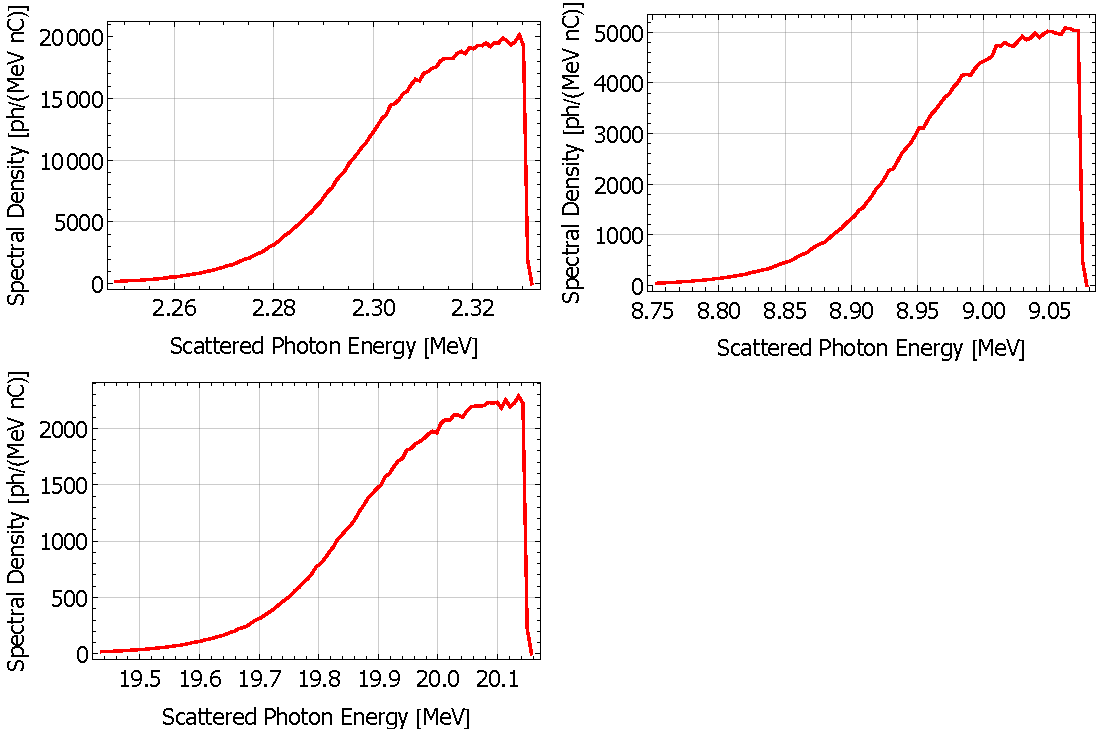
\includegraphics[width=\textwidth]{Figures/DIANA_Inverse_Compton_Source_Design/DIANA_spectra.pdf}
\caption{Predicted spectral output (flux) of 1064~\si{\nano\meter} incident photons interacting head-on ($\phi=0$) with each of the three nominal energy electron bunches in DIANA; this spectrum was generated using the \textsc{ICARUS} code. Top Left: 362~\si{\mega\electronvolt}  electron bunch--laser pulse interaction spectrum, with peak energy $E_{\gamma}=2.33$~\si{\megaelectronvolt} and an angular crossing luminosity reduction factor (Eq.~\ref{eq:angular_crossing_factor}) $R_{AC}=0.143$. Top Right: 717~\si{\mega\electronvolt}  electron bunch--laser pulse interaction spectrum, with peak energy $E_{\gamma}=9.07$~\si{\mega\electronvolt} and an angular crossing luminosity reduction factor  $R_{AC}=0.143$. Bottom Left: 1072~\si{\mega\electronvolt}  electron bunch--laser pulse interaction spectrum, with peak energy $E_{\gamma}=20.13$~\si{\mega\electronvolt} and an angular crossing luminosity reduction factor  $R_{AC}=0.142$.}
\label{fig:DIANA_spectra}
\end{figure}

The spectra of the DIANA ICS source at each of the three nominal energies ($E_{e} = $362, 717, 1072~\si{\mega\electronvolt}) are similar in shape throughout all electron energies however, they differ significantly in both spectral density and scattered photon energy. The scattered photon energies (Eq.~\ref{eq:scattered_photon_energy}) vary due to the $E_{\gamma}\propto\gamma^{2}$ double Doppler shift, where the scattered photon energies at the Compton edge of the spectra agree with the calculated values in Table~\ref{tab:DIANA_spectral_output}. Scattered photon energies above the Compton edge (Eq.~\ref{eq:compton_edge_energy}) are produced because electrons and incident laser photons exist with energy spreads that increase their energy beyond the electron bunch nominal energy and these can interact with each other to produce more energetic scattered photons -- a high scattered photon energy tail. A portion of the total ICS interaction spectrum is selected by the collimator (in this case the 0.5\% \textit{rms} bandwidth), therefore the scattered photon energies are cut-off and a low scattered photon energy tail is observed. The low scattered photon energy tail occurs due to emittance effects and because the photons are not all backscattered ($\theta\neq 0$) -- so lower energy photons are present in the spectrum.   

The peak spectral density of the DIANA ICS sources in the spectrum is decreased as a function of the electron bunch energy as the spectral density (Eq.~\ref{eq:spectral_density}) is inversely proportional to the Lorentz factor squared ($\mathcal{S} \propto 1/\gamma^{2}$), as the spectral density is the flux per unit scattered photon energy and there is a $\gamma^{2}$ dependence in the scattered photon energy (Eq.~\ref{eq:scattered_photon_energy}). To illustrate the spectral density decrease with electron energy, the variation in the peak spectral density of the 362 and 1072~\si{\mega\electronvolt} electron bunch cases ($\mathcal{S}_{\mathrm{pk}}^{362~\si{\mega\electronvolt}}$ and $\mathcal{S}_{\mathrm{pk}}^{1072~\si{\mega\electronvolt}}$) and their variation in Lorentz factor squared can be compared yielding
\begin{align}
\frac{\mathcal{S}_{\mathrm{pk}}^{362~\si{\mega\electronvolt}}}{\mathcal{S}_{\mathrm{pk}}^{1072~\si{\mega\electronvolt}}} &= \frac{20151~\mathrm{ph}/\si{\mega\electronvolt\nano\coulomb}} {2285~\mathrm{ph}/\si{\mega\electronvolt\nano\coulomb}} = 8.82 \nonumber\\
\frac{\gamma_{1072~\si{\mega\electronvolt}}^{2}}{\gamma_{362~\si{\mega\electronvolt}}^{2}} &= \frac{4.41\times 10^{6}}{5.03\times 10^{5}} = 8.77 \nonumber
\end{align}
therefore, it is evident that this is the origin of the decrease in spectral density. The spectra in Fig.~\ref{fig:DIANA_spectra} are not smooth spectra, as shown for the CBETA ICS source in Section~\ref{sec:CBETA_spectral_output}, because the energy spread is very small and causes oscillatory integration errors within the \textsc{ICARUS} code (see Section~\ref{sec:benchmarking_cases_characterisation_optimisation}). The resultant roughness of the DIANA ICS source is non-physical.

The collimated flux resulting from yield calculations of the \textsc{ICARUS} spectra at each nominal electron energy (for 0.5\% \textit{rms} bandwidth), when the crossing angle luminosity reduction factors (Eq.~\ref{eq:angular_crossing_factor}) are reintroduced ($R_{AC} \approx 0.14$, for all nominal electron energies), are
\begin{align}
\mathcal{F}_{\mathrm{col}^{362~\si{\mega\electronvolt}} &= 1.31\times 10^{9}~\mathrm{ph}/\si{\second}} \\
\mathcal{F}_{\mathrm{col}}^{7171~\si{\mega\electronvolt}} &= 1.30\times 10^{9}~\mathrm{ph}/\si{\second} \\
\mathcal{F}_{\mathrm{col}}^{1072~\si{\mega\electronvolt}} &= 1.29\times 10^{9}~\mathrm{ph}/\si{\second}
\end{align}
which are in close agreement with the collimated fluxes calculated analytically (Eq.~\ref{eq:collimated_flux}) in Table~\ref{tab:DIANA_spectral_output}. Small variations are expected between the analytical collimated flux and the collimated flux calculated from \textsc{ICARUS} spectra as the analytical calculation does not account for energy spread of the electron bunch or laser pulse spectral bandwidth. As energy spread of the electron bunch and spectral bandwidth of the laser pulse are very small we see good agreement.

\section{Gamma-ray ICS Source Comparison}
\label{sec:gamma_ICS_comparison}

Inverse Compton scattering sources for production of $\gamma$-rays have been designed and demonstrated worldwide; comparison of the DIANA ICS source against these shows the benefits of the ERL driven ICS approach. Differing approaches for the production of $\gamma$-rays have been trialed such as variations on the type of accelerators and incident photon sources used. For example, the HI$\gamma$S source uses radiation produced from a free electron laser to achieve high energy photon production up to 100~\si{\mega\electronvolt} \cite{weller2009research}. ICS sources may also have different design goals, for example sources may be designed for high peak brilliance, to produce a high flux per shot with a short pulse duration, for destructive inspection of samples. With conventional lasers configurations for the ICS sources can differ, as some sources may favour the high peak brilliance approach of a `single shot' design whereas some favour the `re-circulated pulse' approach leading to high average brilliance, for example for time average measurements such as nuclear resonance fluorescence studies. The two main conventional laser ICS source approaches are detailed in Section~\ref{sec:lasers_fabry_perot}. The most relevant $\gamma$-ray ICS facilities for comparison to the DIANA ICS source are those producing $\gamma$-ray radiation with scattered photon energis on the \si{\mega\electronvolt}-scale ($E_{\gamma}>1$~\si{\mega\electronvolt}); a selection of these sources are tabulated in Table~\ref{tab:gammaray_ICS_comparison}, which presents a combination of operating facilities and recently designed ICS sources. 
\begin{table}[!h]
\caption{Comparison of existing and designed $\gamma$-ray ICS.}
\begin{threeparttable}
\resizebox{\columnwidth}{!}{
\begin{tabular}{lccc}
\hline\hline
ICS & Accelerator Type & Scattered Photon Energy (\si{\mega\electronvolt}) & Flux (ph/\si{\second}) \\
\hline
DIANA\tnote{*} & ERL & 2.33--20.11 & 5.77--6.08$\times 10^{10}$ \\ 
FEBE Exp.\tnote{*}\tnote{$\dagger$} & Linac & $<$1.48 & 4.63--5.83$\times 10^{5}$ \\
NIJI-IV \cite{sei2017demonstration} & Storage Ring & 1.2 & 3.1$\times 10^{4}$ \\
VIGAS\tnote{*} \cite{shi2021vigas,brenner2020summary} & Linac & 0.2--4.8 & 1--4$\times 10^{8}$ \\
ELI-NP-GBS\tnote{*} \cite{adriani2014technical} & Linac & 0.2--19.5 & $3.9\times 10^{9}$ \\
ELI-NP VEGA\tnote{*} \cite{tanaka2020current,elinp2019vega} & Storage Ring & 1--19.5 & 1$\times 10^{11}$\\
NewSUBARU \cite{utsunomiya2015gamma} & Storage Ring & 5--40 & $3\times 10^{7}$ \\
%VELOCIRAPTOR & Linac & & \\
%T-REX & Linac & & \\
Pan et al CBS\tnote{*} \cite{pan2019design} & Storage Ring & 4--10 & 0.14--3.87$\times 10^{12}$ \\ 
Super-ACO \cite{nutarelli1998gamma} & Storage Ring & 33.4 & $5\times10^{6}$ \\
HI$\gamma$S \cite{weller2009research} & Storage Ring & 1--100 & 5$\times 10^{7}$--5$\times 10^{8}$ \\
\hline\hline
\end{tabular}}
\begin{tablenotes}
\item[*]{Denotes design parameters for sources which are not yet demonstrated.}
\item[$\dagger$]{The FEBE ICS experiment is detailed in Chapter~\ref{FEBE_Inverse_Compton_Scattering_Experiment}.}
\end{tablenotes}
\end{threeparttable}
\label{tab:gammaray_ICS_comparison}
\end{table}

% How does DIANA measure up? ENERGY
The DIANA ICS source is designed to produce $\gamma$-rays across a wide range of scattered photon energies ($E_{\gamma}=$2.33--20.11~\si{\mega\electronvolt}), and will be designed to be steplessly variable -- any scattered photon energy in this range will be accessible within this range -- via adjustment of the electron bunch energy. The tunability proposed for the DIANA ICS matches the tunability of the ELI-NP-VEGA system \cite{tanaka2020current,elinp2019vega}. However, other ICS sources such as NewSUBARU and HI$\gamma$S are capable of producing $\gamma$-rays up to 40~\si{\mega\electronvolt} and 100~\si{\mega\electronvolt} respectively, extending the utility of those sources into the nuclear photonics regime \cite{budker2021expanding}. High-energy photon capabilities are possible at NewSUBARU and HI$\gamma$S because of two approaches: the use of frequency doubled lasers at short wavelengths, for example a 2nd harmonic Nd:YAG laser ($\lambda = 532$~\si{\nano\meter}) or using short-wavelength radiation from a FEL. The former approach is implementable within the current design of the suite of ICS sources on DIANA and is suitable for further work, yet use of frequency doubled lasers in Fabry-Perot optical cavities poses additional challenges for high average stored power (see Section~\ref{sec:lasers_fabry_perot}).

% Re-circulation advantage and the abundance of storage ring driven ICS
Table~\ref{tab:gammaray_ICS_comparison} shows that none of the well-known ICS sources designed and operated have utilised the ERL approach and in-depth consideration of an ERL as the driver of an inverse Compton scattering source for production of $\gamma$-rays is limited. Predominantly, ICS $\gamma$-ray production is driven by storage ring methods with existing ICS sources, such as NewSUBARU \cite{utsunomiya2015gamma} and HI$\gamma$S \cite{weller2009research}, utilising existing synchrotron facilities. The european $\gamma$-ray flagship source ELI-NP $\gamma$-ray source plans to utilise the Lyncean Technologies variable energy gamma-ray (VEGA) system \cite{tanaka2020current,elinp2019vega} -- a storage ring system, in favour of the ELI-NP-GBS \cite{adriani2014technical} linac system, so next generation ICS sources are still based on the existing storage ring approach. Storage ring sources are undoubtedly favoured because of the high-flux available due to re-circulation of the electron bunch and laser pulse leading to a higher interaction rate. However, as demonstrated in the DIANA ICS source design, because of re-circulation ERL driven ICS sources are capable of high flux operation as in storage ring driven ICS; further evidenced by the similarity in flux predictions for the DIANA ICS source and leading designs such as ELI-NP VEGA and the CBS \cite{pan2019design} in Table~\ref{tab:gammaray_ICS_comparison}. Therefore, the ERL approach deserves further scrutiny, especially with the advent of multi-turn ERLs (as demonstrated by CBETA \cite{bartnik2020cbeta}) and future high electron energy ERL projects, such as PERLE \cite{angal2018perle} and CEBAF \cite{meot2016er}, as ERLs may offer smaller emittance, energy spread and more brilliant electron beams which constitute a narrowband ICS source.

% How does DIANA measure up? FLUX
Examination of Table~\ref{tab:gammaray_ICS_comparison} show that DIANA is of the same order in flux and scattered photon energy as other world-leading source designs, such as those by Pan et al \cite{pan2019design} and the ELI-NP-VEGA collaboration \cite{elinp2019vega,tanaka2020current}. The DIANA ICS source flux of 6.08$\times 10^{11}$ph/\si{\second} is bested by both the Compton Back-scattering Source (CBS) by Pan et al \cite{pan2019design}, where a factor of 2 larger laser pulse energy is stored, and the ELI-NP-VEGA source, which is also expected to use a higher average stored power cavity (beyond the average stored power of DIANA). Head-on ($\phi=0$) interactions are also assumed in the highest flux sources (ELI-NP-VEGA and CBS); the implementation of these are not adequately explained as it is unclear whether the Fabry-Perot optical cavities in each design will have the electron bunches enter within the cavity (via a dipole bend contained in the cavity) or by using holes in the optical cavity mirrors, both pose issues for optical cavity development as explained in Section~\ref{sec:lasers_fabry_perot}. In the Pan et al CBS design\cite{pan2019design} the hourglass effect -- the effect of diverging electron bunch and laser pulse producing a variable IP spot size -- has been neglected, and this would be non-negligible in the Pan et al \cite{pan2019design} CBS case because the electron bunch and laser pulse are both of considerable length ($\sigma_{z,e} = 110$~\si{\milli\meter}, $\sigma_{z,L} = 6$~\si{\milli\meter}) resulting in an hourglass effect luminosity reduction factor (Eq.~\ref{eq:furman_hourglass_reduction}) of $R_{HG} = 0.66$ (a 34\% reduction in luminosity). The DIANA ICS source is capable of similar flux performance as the ELI-NP-VEGA and CBS sources, with an angular crossing IP arrangement and more conservative laser parameters. 

% ERL advantages in bandwidth
Whilst the ERL approach has been shown to be competitive in terms of flux the real advantage of an ERL driven ICS source may be in achieving a narrow bandwidth and production of a large collimated flux per bandwidth. However, quantifying the bandwidth and the collimated flux per bandwidth is difficult as these values are often not quoted within the literature. Narrow bandwidth is necessary for nuclear physics experiments in the $\gamma$-ray regime for example for determining nuclear material composition of mixed isotopic wastes by nuclear resonance fluorescence \cite{angell2015demonstration} where isotopic signatures may lie close to one another or for exploiting narrow resonances (Pygmy, Giant Dipole etc.) in nuclear photonics \cite{budker2021expanding}. 

However, storage ring driven ICS sources can suffer from large bandwidth due to large energy spread in the electron bunch, for example with an energy spread of $\sim0.1$\% \cite{litvinenko1996intense}, the minimum possible bandwidth of the HI$\gamma$S ICS source is limited to 0.2\% by this factor alone. In ICS sources the main limitation on the bandwidth is due to emittance and divergence effects, therefore large equilibriated emittances in storage rings such as the large natural emittance ($\epsilon_{x} = 350$~\si{\nano\meter}--\si{radian}) in HI$\gamma$S \cite{weller2009research} lead to large divergence terms in the bandwidth. For example, the large electron bunch energy spread and high emittance of the HI$\gamma$S source limits the produced $\gamma$-ray beam to a 2.5--3.5\% \textit{FWHM} bandwidth \cite{weller2009research} for high flux operation. However, certain storage ring operation modes such as non-equilibrum rings \cite{huang1998laser,owen2013nonequilibrium} and low emittance designs such as the CBS \cite{pan2019design} ($\epsilon_{x} = 8.64$~\si{\nano\meter}--\si{\radian}, $\Delta E_{e}/E_{e} = 9.56\times 10^{-4}$) may avoid poor bandwidth due to the emittance term (Eq.~\ref{eq:emittance_term}) of the bandwidth, at the cost of a reduction in average electron beam current and subsequently flux.     

Within an ERL both the electron bunch energy spread and large divergence (emittance) limitations are avoided, for example the DIANA ICS source would be capable of a $\sim10^{-5}$ electron bunch energy spread and a small emittance $\epsilon_{nx} = 0.5$~\si{\milli\meter}--\si{\milli\radian} ($\epsilon_{x} = 0.24$~\si{\nano\meter}--\si{\radian}, $E_{e} = 1072$~\si{\mega\electronvolt}), as seen in Table~\ref{tab:DIANA_electron_beam_design_parameters}. Therefore, an ERL driver may be more conducive to design of a high flux, narrowband ICS source than storage rings though specifically designed or operated storage rings potentially could offer similar performance.

\section{Bremsstrahlung Source Comparison}
\label{sec:bremsstrahlung_comparison}

Bremsstrahlung (breaking radiation) is a process that occurs when a particle (here we consider electrons) is incident upon a solid target; the electron traverses the target with kinetic energy $E_{e}$ and is attracted to the positively charged nuclei of the target or repulsed by the electron cloud in the target material (by the Coulomb force) such that the trajectory of the incident electron is bent, resulting in a loss of kinetic energy $E_{k}$. The energy must be conserved and therefore a photon is emitted with the kinetic energy $E_{\gamma}=E_{k}$ lost by the incident electron. A simple schematic of the process is shown in Fig.~\ref{fig:bremsstrahlung_diagram} For example, consider a 50~\si{\mega\electronvolt} electron bunch bombarding a Tungsten (Z = 74) target, at the extremes of the bremsstrahlung process the trajectory of electrons within the bunch may be bent by the target such that all the kinetic energy of the electron is lost and a photon of energy $E_{\gamma}=E_{e}$ is produced or the electrons may traverse the target with an unchanged trajectory where no photon is produced $E_{\gamma}=0$. Bremsstrahlung therefore generates a continuous spectrum of photon energies within the range $0 \leq E_{\gamma} \leq E_{e}$.
\begin{figure}[!h]
\centering
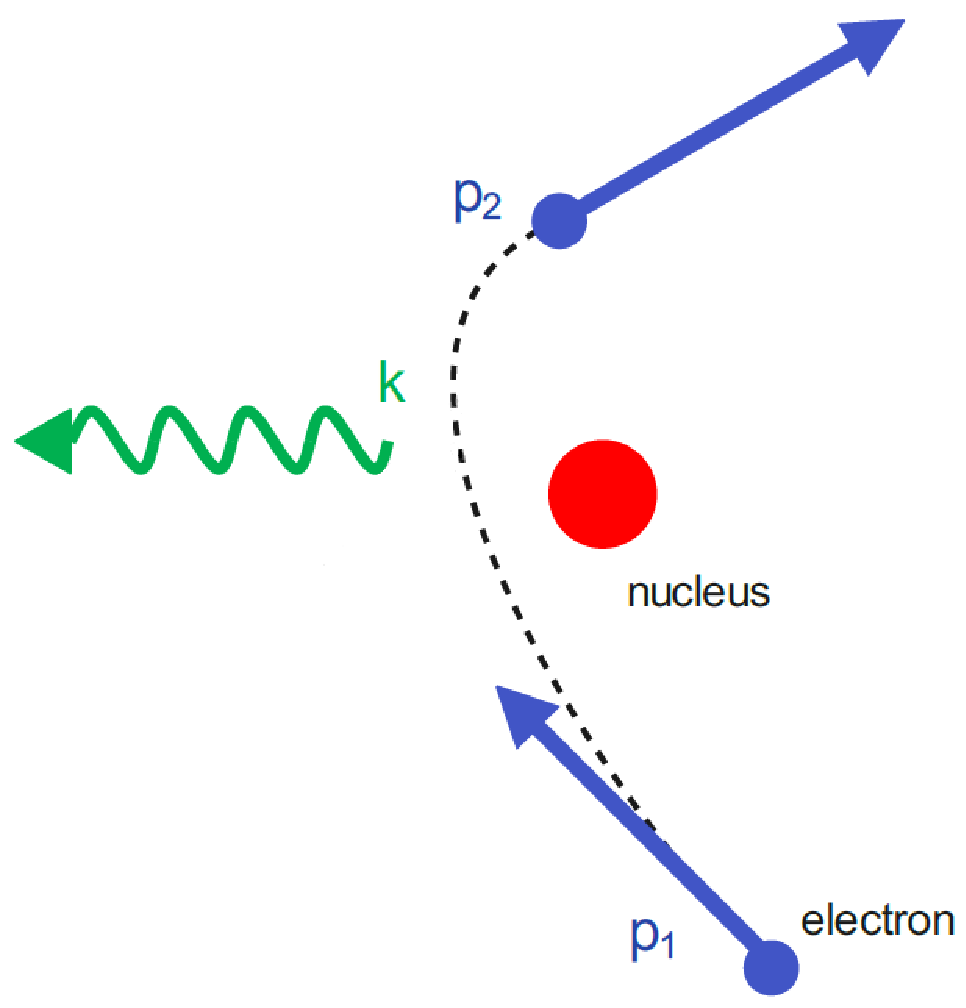
\includegraphics[width=0.5\textwidth]{Figures/DIANA_Inverse_Compton_Source_Design/Bremsstrahlung_fixed.pdf}
\caption{Diagram of the bremsstrahlung process where an electron (blue) with momentum $p_{1}$ is bent from its original trajectory by the Coulomb attraction of a nearby nucleus (red), the momentum of the electron is modified $p_{2}$ and a photon (green) of momentum $\hbar k$ is generated, with energy equal to the kinetic energy reduction of the electron.}
\label{fig:bremsstrahlung_diagram}
\end{figure}

Bremsstrahlung sources are typically more simple to construct than ICS sources -- since a particle beam need only be incident on a stationary target not a counter propagating laser pulse -- and are therefore cheaper. As bremsstrahlung generates photons with energies up to maximum kinetic energy of the particle bunch incident on the target, \si{\mega\electronvolt}-scale photons are available with much lower electron energies. For example, 1~\si{\mega\electronvolt} $\gamma$-rays can be produced by inverse Compton scatteriang via an interaction of an Nd:YAG ($\lambda = 1064$~\si{\nao\meter}) incident laser and a $\sim 235$~\si{\mega\electronvolt} electron bunch in comparison to a bremsstrahlung source where 1~\si{\mega\electronvolt} $\gamma$-rays are readily available from a 5--10~\si{\mega\electronvolt} electron bunch incident on a tungsten target. Therefore, \si{\mega\electronvolt}-scale photons from a bremsstrahlung source can be produced by an accelerator of a portable size using only a converter target and an electron
accelerator \cite{chin2021application}, whereas a large electron accelerator is required for an ICS source operating at similar energies.

However, unlike the ICS process there is no inherent photon energy--angle correspondence ($E_{\gamma}\neq f\left(\theta\right)$), therefore energies of photons can not be simply selected by a collimator. In bremsstrahlung sources photon energy selection is not readily achievable; the spectrum may be narrowed by attenuating the bremsstrahlung photons through material as lower energy photons would be attenuated to a greater extent than the higher energy photons but some would still remain and the attenuation would distort the spectrum overall whilst reducing photon fluxes. Unavoidably bremsstrahlung production of photons over a broad range of energies delivers unnecessary dose that in some cases also interferes with the signature to be detected \cite{geddes2017impact}. The signal-to-noise ratio of the investigated process is reduced, therefore monoenergetic sources allow the sensitivity of a detection system to be improved \cite{jones2008bremsstrahlung}.

The DIANA ICS source may be compared to a bremsstrahlung source to illustrate the monochromaticity of an ICS source spectrum in comparison to the continuous spectrum of a bremsstrahlung source, as shown in Fig.~\ref{fig:ICS_Brem_comparison}. The bremsstrahlung source is based upon an ELEKTA SL linac \cite{hansen1998quality} with an electron bunch energy of 15~\si{\mega\electronvolt} and \textit{rms} energy spread of 1.77\% incident upon a 1~\si{\milli\meter} thick tungsten target, as used by Vagena and Stoulos \cite{vagena2017photodisintegration} to measure the photodisintegration cross section of dysprosium isotopes. The spectrum of the bremsstrahlung source has been simulated using a \textsc{GEANT4} \cite{agostinelli2003geant4} model, where the tungsten target, collimation and filtering system and linac are accounted for. The 362~\si{\mega\electronvolt} nominal electron energy DIANA ICS spectrum, optimised optimised for a 0.5\% \texit{rms} bandwidth (as shown in Fig.~\ref{fig:DIANA_spectra}) is used as the ICS case. Both plots are normalised as the DIANA ICS source is re-circulated and has an incomparably higher flux than the commercial bremsstrahlung source.
\begin{figure}[!h]
\centering
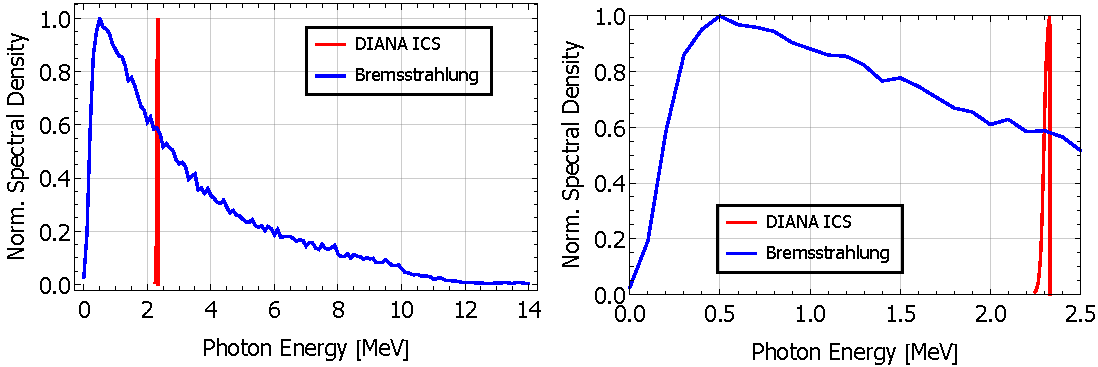
\includegraphics[width=\textwidth]{Figures/DIANA_Inverse_Compton_Source_Design/ICS_Brem_Comparison.pdf}
\caption{}
\label{fig:ICS_Brem_comparison}
\end{figure}

The Elekta linac bremsstrahlung source has a peak photon energy of 0.5~\si{\mega\electronvolt} whereas the peak scattered photon energy of the DIANA ICS source is 2.33~\si{\mega\electronvolt}, as shown in Table~\ref{tab:DIANA_spectral_output}. In Fig.~\ref{fig:ICS_Brem_comparison}, it is evident that the bandwidth of the ICS source is much smaller than the bremsstrahlung source, therefore an ICS source can provide a monochromatic source of photons in comparison to the bremsstrahlung source. Consequently, the DIANA ICS source and ICS sources more generally can perform experiments with an improved targetting of specific resonances and an overall better signal-to-noise ratio.

\textcolor{blue}{**FLUX ARGUMENT - CONVENTIONAL SOURCES**}

Laser plasma wakefield accelerators \cite{sprangle1988laser,esarey2009physics}, have been considered for compact (small accelerator footprint) bremsstrahlung generation of $\gamma$-rays \cite{cipiccia2012tuneable,lemos2018bremsstrahlung}. A discussion of laser wakefield acceleration is not included here, but a comprehensive discussion is presented by Esarey et al \cite{esarey2009physics}. Cipiccia et al \cite{cipiccia2012tuneable} used a Ti:Sa laser ($\lambda = 800$~\si{\nano\meter}) with pulse energy 2.5--3.5~\si{\joule} and laser pulse duration 60--80~\si{\femto\seconds} FWHM to generate 20--25~\si{\pico\coulomb} electron bunches with energies in the range 200--400~\si{\mega\electronvolt} and an \textit{rms} energy spread of 8\%. The 20--25~\si{\pico\coulomb} electron bunches were incident upon a 2~\si{\centi\meter} Aluminium target generating $1\times 10^{9}$ bremsstrahlung photons with photon energies up to $\sim 220$~\si{\mega\electronvolt} and a mean energy of 10~\si{\mega\electronvolt}. A photon flux of $1\times 10^{9}$~ph/\si{\second} is a factor of $\sim 61$ smaller than the flux of the DIANA ICS source in Table~\ref{tab:DIANA_spectral_output}, therefore LWFA bremsstrahlung sources are competitive in terms of photon flux, though this is incomparable with the high flux in a narrow bandwidth ($\mathcal{F}_{\mathrm{0.5\%}} = 1.30\times 10^{9}$~ph/\si{\second}, 0.5\% \textit{rms} bandwidth) achievable from DIANA.    

\section{DIANA ICS Applications}
% Say only certain examples chosen, not comprehensive

A series of ICS sources driven by the 3-turn ERL DIANA would enable a broad range of experiments within nuclear photonics \cite{nedorezov2017nuclear,budker2021expanding} and the nuclear sector such as nuclear resonance fluorescence (NRF) and transmutation toward nuclear forensics and security as well as fundamental nuclear physics such as photonuclear cross section measurements \cite{renstrom2018verification}.
Other wider physics experiments can be performed in fields such as high energy astrophysics, high energy physics and fundamental tests of quantum mechanics, as well as medical isotope production. The DIANA ICS source, with spectral output parameters shown in Table~\ref{tab:DIANA_spectral_output}, offers high flux and a narrow bandwidth which are required for experimentation in these areas, and allows for greater precision measurement than previous sources, as discussed in Section~\ref{sec:gamma_ICS_comparison}. The preliminary examination of applications for the DIANA ICS has focused upon nuclear resonance fluorescence, transmutation of radioactive wastes and photonuclear medical isotope production -- areas in which a high average brilliance, narrowband $\gamma$-ray source can excel.  

\subsection{Nuclear Resonance Fluorescence}

Nuclear resonance fluorescence is a process first described by Kneissl et al \cite{kneissl1996investigation}, where a nucleus of an atom resonantly absorbs a $\gamma$-ray exciting the nucleus to a higher energy excited state, then the nucleus subsequently decays from the excited state, via emission of a $\gamma$-ray, to a lower energy state (ground state or lower excited state). Applied to a bulk sample, with a beam of $\gamma$-rays, the $\gamma$-rays emitted via NRF are distributed homogeneously (i.e. uniform angular distribution) and the energy of the $\gamma$-rays is characteristic to the particular isotope that is being resonantly excited, therefore NRF is applicable to isotopic determination of samples. Nuclear resonance fluorescence is the nuclear (isotopic) analog of x-ray resonance fluorescence (as described in Section~\ref{sec:CBETA_ICS_applications}) used for atomic (elemental) discrimination of samples.  

Nuclear resonance fluorescence was initially applied to the detection of nuclear materials for security purposes such as the detection of clandestine nuclear material \cite{bertozzi2005nuclear,pruet2006detecting,geddes2017impact} for non-proliferation. Then subsequently applied to the assay and identification of nuclear waste \cite{hayakawa2010nondestructive,angell2015demonstration,bolind2015states} and for imaging of manufacturing defects in reactor fuel. Both bremsstrahlung and inverse Compton scattering sources of $\gamma$-rays have been utilised to provide the incident $\gamma$-ray beam for NRF experimentation and a schematic diagram of a NRF experiment utilising an ICS source is shown in Fig.~\ref{fig:NRF_diagram}.

\begin{figure}[!h]
\centering
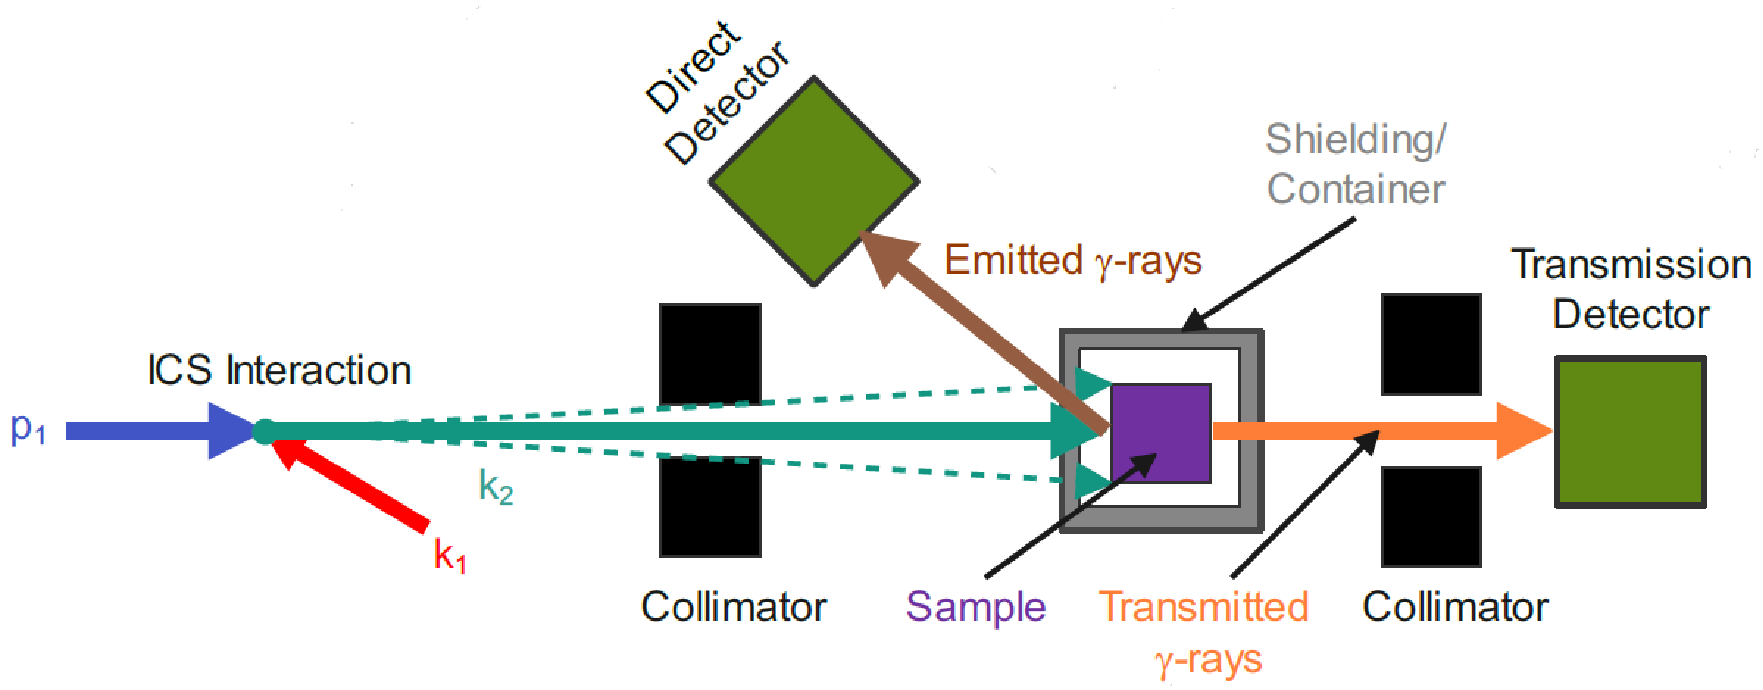
\includegraphics[width=\textwidth]{Figures/DIANA_Inverse_Compton_Source_Design/NRF_diagram_fixed.pdf}
\caption{Diagram of a nuclear resonance fluorescence experiment using a $\gamma$-ray beam (turquoise) generated by an ICS source. A relativistic electron bunch (blue) of momentum $p_{1}$ is interacted with an incident photon pulse (red) of momentum $\hbar k_{1}$ to scatter a $\gamma$-ray photon beam of momentum $\hbar k_{2}$, which is collimated (black) for narrow bandwidth and passed through a shielded (grey) sample (purple).  For transmission measurements the $\gamma$-ray beam is detected by a downstream on-axis detector, after photons are absorbed by the sample at the resonant excitation energies. Direct measurements are conducted by sampling the $\gamma$-rays emitted from the sample from the de-excited states by an off-axis detector.}
\label{fig:NRF_diagram}
\end{figure}

The intrinsic resonance width of the excited state in the nucleus is of the order \si{\milli\electronvolt} to \si{\electornvolt}, and is further broadened to several \si{\electronvolt} by Doppler broadening of nuclear resonances \cite{angell2015demonstration}, which occurs due to the thermal motion of the nuclei in the target material. Therefore, direct probing of just the resonance width would require a $\gamma$-ray beam probe with energy spread on the order of several electronvolts which, with resonances excited on the \si{\mega\electronvolt}-scale, would require a bandwidth on the order of $\Delta E_{\gamma}/E_{\gamma} = 10^{-6}$. Production of $\gamma$-rays with bandwidth on the $10^{-6}$ scale has not been demonstrated, to the authors knowledge, therefore a different approach is required.

A single nuclear resonance may be probed if the energy spread of the $\gamma$-ray pulse is smaller than the energy variation between it's nearest-neighbour resonances. For example, consider the three lowest (and closest in excitation energy) measured excited states of uranium 238, where resonances can be excited with 2.176~\si{\mega\electronvolt}, 2.209~\si{\mega\electronvolt} and 2.245~\si{\mega\electronvolt} $\gamma$-rays respectively \cite{quiter2011transmission}. A $\gamma$-ray beam probe can excite only the 2.209~\si{\mega\electronvolt} resonance if the $\gamma$-ray has a central energy of 2.209~\si{\mega\electronvolt} and the total energy spread of the $\gamma$-ray beam is less than $\Delta E_{\gamma} = 33$~\si{\kilo\electronvolt} (a FWHM value of 25.9~\si{\kilo\electronvolt}) and therefore the FWHM bandwidth of the $\gamma$-ray beam must be $\Delta E_{\gamma/E_{\gamma}} = 0.0117$ i.e a 1.17\% FWHM (0.5\% \textit{rms}) bandwidth. In mixtures of radioisotopes, such as in unknown nuclear waste repositories, the analysis becomes more complex. 

Nuclear resonance fluorescence measurements have been accomplished with both bremsstrahlung \cite{bertozzi2005nuclear} and inverse Compton scattering \cite{angell2015demonstration} $\gamma$-ray sources. Bremsstrahlung has a continuous spectrum, as shown in Section~\ref{sec:bremsstrahlung_comparison}, therefore single nuclear resonances may not be probed and the spectrum of emitted radiation from the NRF assayed sample with have multiple radiation peaks, which are more challenging to discriminate -- especially in poly-isotopic samples. However, ICS sources such as DIANA are capable of narrow bandwidth $\gamma$-ray beam generation and can therefore be used to target single resonances, therefore ICS sources are more suited to NRF experiments.  

Measurements of samples via NRF can be conducted using two methods: transmission and direct, as shown in Fig.~\ref{fig:NRF_diagram}. Direct measurement involves a detector placed at an angle off-axis from the $\gamma$-ray beam, and measures the homogeneously emitted $\gamma$-rays from the decaying excited states. Sample material can be identified with the use of a reference isotope, or reference spectra and quantification of the material is achieved similarly via comparison of the intensity of the emitted $\gamma$-rays with reference material \cite{angell2015demonstration}. Transmission measurements place the detector on-axis with reference to the $\gamma$-ray beam, sampling the incident $\gamma$-rays that pass through the detector but $\gamma$-rays with energies corresponding to the excitation energies of the nuclei are absorbed, leaving a reduction in intensity at these $\gamma$-ray energies known as notches. The energies of the notches allow for identification of the sample material and the depth of the notches, in comparison to reference material, allows for quantification \cite{pruet2006detecting}. Transmission measurements are typically quicker as the full absorption of $\gamma$-rays is sampled whereas in a direct measurement only a select solid angle of the emitted photons are detected, so only part of the emission is sampled.

The first nominal electron kinetic energy ($E_{e} = 362$~\si{\mega\electronvolt}) of the DIANA ICS source is capable of producing tunable $\gamma$-rays with a centroid energy of 2.33~\si{\mega\electronvolt}, which is useful for nuclear resonance fluorescence based assays of fissile materials as fissile materials have strongly excited energy levels at 2--3\si{\mega\electronvolt} \cite{angell2015demonstration}. Strongly excited levels occur at 2--3~\si{\mega\electronvolt} in isotopes such as uranium because of the scissor modes of nuclei \cite{iudice1978new,bohle1984new} -- where, in a deformed nucleus, the protons and neutrons oscillate out of plane to each other. A high flux source such as DIANA would also be useful in reducing the measurement time of nuclear resonance fluorescence studies, which is proportional to the number of incident $\gamma$-rays, as the flux of DIANA is 110 times larger than HI$\gamma$S \cite{weller2009research}.

For example, the three isotopes of high importance in nuclear nonproliferation are $^{238}\mathrm{U}$, $^{235}\mathrm{U}$ and $^{239}\mathrm{Pu}$, which display major resonances for incident photon energies of $E_{238~U}^{\mathrm{NRF}} = 2.176$~\si{\mega\electronvolt} \cite{quiter2011transmission},  $E_{235~U}^{\mathrm{NRF}} = 1.733$~\si{\mega\electronvolt} and  $E_{239~Pu}^{\mathrm{NRF}} = 2.143$~\si{\mega\electronvolt} \cite{hayakawa2010nondestructive}. Tuning the electron bunch energy of DIANA in the first turn within the electron energy range $E_{\gamma} =$ 312--350~\si{\mega\electronvolt} allows studies of these isotopes. Using a similar comparison to that employed for spacing between uranium 238 resonances, we see that the difference between $^{238}\mathrm{U}$ \cite{quiter2011transmission} and $^{239}\mathrm{Pu}$ \cite{hayakawa2010nondestructive} resonances is often on the order of $\sim10--100$~\si{\kilo\electronvolt} -- achievable with DIANA. Therefore, a narrowband source with tunability of both the scattered photon energy (Eq.,~\ref{eq:scattered_photon_energy}) and the bandwidth of the $\gamma$-ray beam (Eq.~\ref{eq:RMS_bandwidth}) is a requirement for isotopic determination by NRF. DIANA, if designed to be steplessly variable in $\gamma$-ray scattered photon energy, with adjustable electron bunch focusing and collimation would be an ideal ICS source to provide the required $\gamma$-ray beam for nuclear resonance fluorescence studies.  

In addition, collective modes of nuclei such as giant dipole resonances \cite{goldhaber1948nuclear,baldwin1947photo}, pygmy dipole resonances \cite{cook1957photodisintegration,tonchev2010spectral} and scissor modes \cite{iudice1978new,de1984reformulation,bohle1984new} can be probed via NRF techniques using $\gamma$-ray ICS sources. Collective modes of nuclei study the oscillations of the nucleons within a nucleus, for example giant dipole resonances occur when the protons and neutrons in a nucleus oscillate around their equilibrium positions with respect to each other forming an electric dipole mode. Excitation of these collective modes can be useful to nuclear structure studies.

An example of NRF studies of collective modes of nuclei is the study of the M1 scissors mode of a $^{152}\textrm{Sm}$ nucleus, which has recently been probed at the HI$\gamma$S source to investigate the electric quadrupole (E2) mode decay \cite{ide20212}. However, this experiment was limited by the large 100~\si{\kilo\electronvolt} \textit{FWHM} bandwidth \cite{ide20212} of the source at the $E_{\gamma} = 2.995$~\si{\mega\electronvolt} incident $\gamma$-ray energy required to probe the scissor mode \cite{ziegler1993low} and consequently excited states beyond the $2^{+}$ state are inaccessible because of the insensitivity of the incident $\gamma$-ray beam \cite{ide20212}.

However, the DIANA ERL ICS source using a 362~\si{\mega\electronvolt} electron bunch ($E_{\gamma} =$ 2.33~\si{\mega\electronvolt}) produces a $\gamma$-ray beam with a textit{FWHM} energy spread of 25.9~\si{\kilo\electronvolt} -- a factor $\sim4$ smaller than the HI$\gamma$S bandwidth. Therefore, higher precision nuclear physics experiments may be available with the DIANA ICS source. The DIANA ICS source is also designed to produce comparatively larger flux than HI$\gamma$S, as seen in Table~\ref{tab:gammaray_ICS_comparison}, which will improve data acquisition times for these measurements. Improvements in flux and bandwidth with respect to HI$\gamma$S \cite{weller2009research} in DIANA are also present in ELI-NP-VEGA \cite{elinp2019vega}, where the ELIADE research program aims to distinguish and separate different excitations in the overlapping region of the pygmy dipole resonance (PDR), the giant dipole resonance (GDR), the magnetic dipole resonance (MDR), and the pygmy quadrupole resonance (PQR) \cite{tanaka2020current}. Experiments in these fields would therefore also be suitable for the DIANA ICS source.

\subsection{Transmutation of Nuclear Waste}
% IMPROVE + EXTEND
Progressing towards the higher energy $\gamma$-rays ($E_{\gamma} =$ 9.06--20.11~\si{\mega\electronvolt}) produced via a DIANA ICS source operating at the 2nd and 3rd turn nominal electron bunch kinetic energy (717, 1072~\si{\mega\electronvolt}) of DIANA, studies such as transmutation of waste and fission dynamics become plausible. Photonuclear transmutation reactions such as $(\gamma,p)$, $(\gamma,n)$, $(\gamma,\alpha)$, $(\gamma,f)$ become possible above 5~\si{\mega\electronvolt} which, when driven by suitable fluxes of photons \textcolor{blue}{**NUMBER?**}, could potentially transform long-lived wastes such as $^{241}\mathrm{Am}$ and $^{129}\mathrm{I}$ into wastes with shorter lifespan or wastes that are easier to handle. 

For example, $^{129}\mathrm{I}$ is a major long lived waste with half-life $T_{1/2} = 1.57\times 10^{8}$~\si{\years}, which poses an additional challenge to repository storage methods \cite{cho2016reconsideration} due to water solubility. Whilst other storage methods are being developed \cite{lee2021chemical,morizet2021immobilization}, another solution would be transmutation of this waste to a stable state, as proposed by Rehman et al \cite{ur2017optimization}, using a giant dipole resonance photonuclear reaction ($\gamma$,n) 
\begin{equation}
^{129}\mathrm{I} \left(T_{1/2}=1.57\times 10^{7}\textrm{y}\right) \xrightarrow[]{\left(\gamma,n\right)} {}^{128}\mathrm{I} \left(T_{1/2}=24.99\mathrm{\si{\minute}}\right) \substack{\xrightarrow[]{\left(\beta^{-},93.1\%\right)} {}^{128}\mathrm{Xe}\left(\mathrm{stable}\right)\\[0.1em] \xrightarrow[]{\left(\beta^{+},6.9\%\right)} {}^{128}\mathrm{Te}\left(\mathrm{stable}\right)}
\label{eq:129I_photonuclear_transmutation}
\end{equation}
where $^{129}\mathrm{I}$ is transmuted to two stable isotopes $^{128}\mathrm{Xe}$ and $^{128}\mathrm{Te}$. Based on the cross section measurements for $^{129}\mathrm{I}$ by J. Magill et al \cite{magill2003laser}, as re-created in Fig~\ref{fig:I129_cross_section_photon_energy} using data from the EXFOR database entry \cite{zerkin2018experimental}, the peak cross section of the photonuclear reaction is $\sigma_{\mathrm{reac}} = 229$~\si{\milli\barn} at 15~\si{\mega\electronvolt}. Tuning DIANA to the required 15~\si{\mega\electronvolt} scattered photon energy would produce a total of $6.04\time 10^{10}$~ph/\si{\second} which, when scaling the transmutation rate with the assumed $10^{13}$~ph/\si{\second} quoted by Rehman et al \cite{ur2017optimization}, would produce a transmutation rate of $\sim10^{8}$~atoms/\si{\second}. Therefore, only miniscule amounts ($\sim0.1$~\si{\micro\gram}) could be processed within a year by this method but there is scope for proof of principle experiments.  

\begin{figure}[!h]
\centering
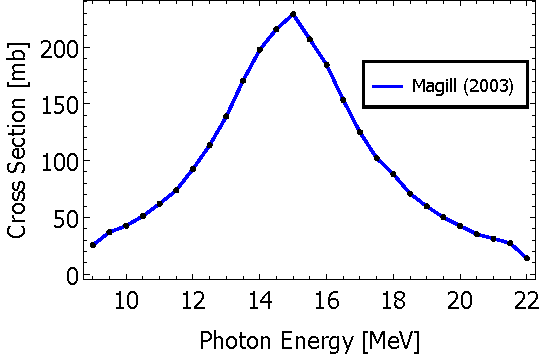
\includegraphics[width=0.7\textwidth]{Figures/DIANA_Inverse_Compton_Source_Design/Iodine_129_cs_photon_energy.pdf}
\caption{Measured \cite{magill2003laser} photonuclear GDR $\left(\gamma,n\right)$ cross section as a function of incident photon energy for the long-lived radioactive waste isotope $^{129}\mathrm{I}$. The cross section peaks at $E_{\gamma} = 15$~\si{\mega\electronvolt} incident photon energy with a cross section of $\sigma = 229$~\si{\milli\barn}. Data acquired from EXFOR database \cite{zerkin2018experimental}.}
\label{fig:I129_cross_section_photon_energy}
\end{figure}

\subsection{Photonuclear Medical Isotope Production}
\label{sec:photonuclear_medical_isotope_production}

\textcolor{blue}{**BLURB ABOUT MEDICAL ISOTOPES, TREATMENT, IMAGING, THERANOSTIC etc.**\\**PRODUCTION METHODS - REACTOR, CYCLOTRON**}

Radionuclides have abundant uses within the realms of medical treatment, with application in imaging, such as $\beta^{+}$ emitting isotopes like $^{18}\mathrm{F}$ with wide use from tumour volume imaging studies \cite{rocha2021metabolic} to investigations of long Covid-19 \cite{sollini2021long}, in treatment, such as prostate cancer brachytherapy \cite{yuan2021proof} with $^{192}\textrm{Ir}$ ($T_{1/2} =73.83$~\si{\day}, $\beta^{-}$, 95.13\%, $\epsilon$, 4.87\%). Theranostic \cite{svenson2013theranostics} radionuclide treatments, where isotopes or combinations thereof find use within joint imagining and treatment, have became a recent focus in this area of research. For example, $^{64}\mathrm{Cu}$ is a theranostic isotope which decays through $\beta^{+}$ (61\%) and $\beta^{-}$ (39\%) with the emission of Auger electrons \cite{boschi2018emerging}; allowing simultaneous diagnostic imaging and therapy with the same radio-pharmaceutical.

A range of production methods for medical isotopes are available such as cyclotron based production \cite{} with $\left(p,x\right)$ reactions, research reactor production \cite{} with $\left(n,x\right)$ reactions, isotope separation on-line (ISOL) production with $\left(p,f\right)$ reactions \cite{} as well as the photonuclear production methods with $\left(\gamma,x\right)$ reactions \cite{habs2011production}. \textcolor{blue}{**NO CARRIER ADDED PRODUCTION, WHY ISOL IS GOOD (MASS SPEC), WHY PHOTONUCLEAR IS GOOD (NARROWBAND)}. 

Using the DIANA ICS source, with high flux and narrow bandwidth, preliminary experiments on the photonuclear production of medical isotopes could be undertaken. A series of candidates have been evaluated for production using DIANA, with particular focus on the photoneutron $\left(\gamma,n\right)$ reaction. Within this section photonuclear production of two promising medical isotope candidates: $^{153}\mathrm{Sm}$ and $^{155}\mathrm{Tb}$ will be investigated.  

\subsubsection{Samarium 153 Production}

Samarium 153 is a well established radionuclide used in the commercial radio-pharmaceuticals Quadramet \cite{ema2015quadramet} -- Samarium lexidronam pentasodium -- which via $\beta^{-}$ decay 
\begin{equation}
^{153}\mathrm{Sm} \left(T_{1/2} = 1.93~\mathrm{\si{\day}}\right)\xrightarrow[]{\left(\beta^{-},\mathrm{100\%}\right)} {}^{153}\mathrm{Eu},
\label{eq:153Sm_beta_minus_decay}    
\end{equation}
is used as a therapy for palliation of bone metastases \cite{kapoor2021cancer,murray2021systemic}. Typically, $^{153}\mathrm{Sm}$ is produced in a research reactor via 
\begin{align}
^{152}\mathrm{Sm}&\xrightarrow[]{\left(n,\gamma\right)}{}^{153}\mathrm{Sm} \\
^{154}\mathrm{Sm}&\xrightarrow[]{\left(n,2n\right)}{}^{153}\mathrm{Sm}
\label{eq:153Sm_research_reactor_production}
\end{align}
neutron capture reactions using highly enriched Samarium targets. Enriched $^{152}\mathrm{Sm}$ and $^{154}\mathrm{Sm}$ targets can be produced using electromagnetic isotope separators which has been demonstrated at Oak Ridge Laboratory using Caultrons producing enrichments of $>$98\% respectively \cite{bell1987stable}. These highly enriched Samarium isotope targets are now available commercially at enrichments of $>$98.4\% and $>$98.5\% \cite{isoflex2021sm}. However, due to the relatively short half-life of $^{153}\mathrm{Sm}$ ($T_{1/2} = 1.93$~\si{\day}) and the neutron rich environment of a reactor, research reactor irradiation production methods are suceptible to contamination with $^{154}\mathrm{Eu}$ \cite{naseri2021effective,van2018separation} via
\begin{equation}
^{153}\mathrm{Sm}\xrightarrow[]{\left(\beta^{-},\mathrm{100\%}\right)}{}^{153}\mathrm{Eu}\xrightarrow[]{\left(n,\gamma\right)}{}^{154}\mathrm{Eu},
\label{eq:153Sm_reactor_contamination}    
\end{equation}
typically occurs where the $^{153}\mathrm{Sm}$ $\beta^{-}$ decays during irradiation to $^{153}\mathrm{Eu}$ which then undergoes neutron capture $\left(n,\gamma\right)$ to $^{154}\mathrm{Eu}$. The $^{154}\mathrm{Eu}$ contaminant is relatively long-lived ($T_{1/2} = 8.59$~y), which results in difficulties for storage and handling of $^{153}\mathrm{Sm}$ based radiopharmaceuticals and a short 24 hour shelf-life \cite{ema2015quadramet} as the prevalence of $^{154}\mathrm{Eu}$ impurities becomes too high \cite{van2018separation}.

However, photonuclear production of $^{153}\mathrm{Sm}$ \cite{carlos1974giant,filipescu2014photoneutron} is possible via
\begin{equation}
^{154}\mathrm{Sm}\xrightarrow[]{\left(\gamma,n\right)}{}^{153}\mathrm{Sm},
\label{eq:153Sm_photonuclear_production}    
\end{equation}
using an ICS $\gamma$-ray source such as DIANA and a highly enriched ($>$98\%) $^{154}\mathrm{Sm}$ target \cite{bell1987stable,isoflex2021sm}. There are several competing photonuclear processes alongside the pathway targeted in (Eq.~\ref{eq:153Sm_photonuclear_production}) such as \cite{carlos1974giant}
\begin{align}
^{154}\mathrm{Sm}\xrightarrow[]{\left(\gamma,2n\right)}{}^{152}\mathrm{Sm},\\
^{154}\mathrm{Sm}\xrightarrow[]{\left(\gamma,n\right)+\left(\gamma,np\right)}{}^{153}\mathrm{Sm}+{}^{152}\mathrm{Pm},
\label{eq:153Sm_photonuclear_disruptors}    
\end{align}
for a mono-isotopic $^{154}\mathrm{Sm}$ target. More competing processes may occur, such as a $\left(\gamma,3n\right)$ reaction etc. however data for these is unavailable in the EXFOR database \cite{zerkin2018experimental} and the literature, we limit this discussion to the measured cross-sections. A full study of impurities would be required, but this is beyond the scope of this investigation.   The cross section of the desired (Eq.~\ref{eq:153Sm_photonuclear_production}) and measured disruptive (Eq.~\ref{eq:153Sm_photonuclear_disruptors}) photonuclear processes as a function of $\gamma$-ray photon energy in Fig.~\ref{fig:154Sm_cross_section_photon_energy}.

\begin{figure}[!h]
\centering
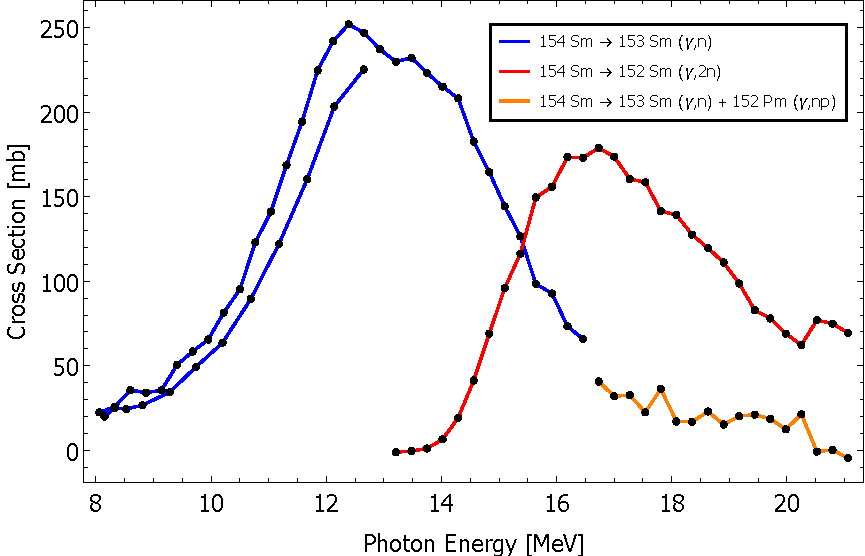
\includegraphics[width=0.8\textwidth]{Figures/DIANA_Inverse_Compton_Source_Design/Sm154Landscape.pdf}
\caption{Reaction cross section against incident photon energy for the $^{154}\mathrm{Sm} \left(\gamma,n\right)$ reaction of interest (blue, higher data \cite{carlos1974giant}, lower data \cite{filipescu2014photoneutron}), and the potentially disruptive reactions $^{154}\mathrm{Sm} \left(\gamma,2n\right)$ (red \cite{carlos1974giant}) and $^{154}\mathrm{Sm} \left(\gamma,n\right) + \left(\gamma,np\right)$ (orange \cite{carlos1974giant}). Data for other reactions photonuclear reactions involving $^{154}\mathrm{Sm}$ was unavailable. Data acquired from the EXFOR database \cite{zerkin2018experimental}. }
\label{fig:154Sm_cross_section_photon_energy}
\end{figure}

In Fig.~\ref{fig:}, two measurements of the $^{154}\mathrm{Sm}\left(\gamma,n\right)$ cross section are made by Filipescu et al \cite{filipescu2014photoneutron} using the NewSUBARU $\gamma$-ray source \cite{utsunomiya2015gamma} and Carlos et al \cite{carlos1974giant} where monochromatic $\gamma$-rays were generated using in-flight positron annihilation \cite{miller1960monochromatic}, where a positron beam impinges upon a target, in a 60~\si{\mega\electronvolt} linac at Saclay \cite{audit1970etude}. In-flight positron annihilation methods produce both a narrowband radiation spectral line resulting from positron--electron the annihilations in the target as well as the typical Bremsstrahlung radiation spectrum; the two can't be disentangled, but the ratio of the signal of the positron annihilation to the Bremsstrahlung spectrum can typically be maximised through use of a small collimation angle resulting in collimated fluxes of $1.5\times10^{3}$~ph/\si{\second} and \textit{FWHM} bandwidths of $\sim 12$\% for the upgraded Saclay source \cite{veyssiere1979quasi}. Comparing the Saclay positron source with the NewSUBARU ICS source in Table~\ref{tab:gammaray_ICS_comparison} and using the approximation $\mathcal{F}_{\mathrm{0.1\%}} = 1.5\times 10^{-3}\mathcal{F}$ \cite{krafft2010compton}, the flux for the NewSUBARU ICS source would be higher than the upgraded Saclay positron annihilation source \cite{veyssiere1979quasi} therefore this measurement has a better signal to noise ratio and the \textit{FWHM} bandwidth of NewSUBARU is 1-2\%, a factor of 6 improvement on the Saclaay upgraded source. Therefore, the NewSUBARU $^{153}\mathrm{Sm}\left(\gamma,n\right)$ measurement offers superior precision. 


Fig.~\ref{fig:154Sm_cross_section_photon_energy} shows that the known competing processes for a mono-isotopic $^{154}\mathrm{Sm}$ can be avoided below 13.21~\si{\mega\electronvolt} as this is the threshold for the $^{154}\mathrm{Sm}\left(\gamma,2n\right)$ photonuclear reaction. However, some of the data presented by Carlos et al \cite{carlos1974giant} for the disruptive processes has negative cross sections, which appears to be unphysical. The peak cross sections for the desired $^{154}\mathrm{Sm}\left(\gamma,n\right)$ reaction are $\sigma_{\mathrm{reac}} = 252.1$~\si{\milli\barn} at $E_{\gamma} = 12.39$~\si{\mega\electronvolt} (Carlos et al \cite{carlos1974giant}) and $\sigma_{\mathrm{reac}} = 225.3$~\si{\milli\barn} at $E_{\gamma} = 12.65$~\si{\mega\electronvolt} (Filipescu et al \cite{filipescu2014photoneutron}). Therefore, with the DIANA ICS source tuned to the scattered photon energy corresponding to the peak cross section, photonuclear production of $^{153}\mathrm{Sm}$ is possible.

The specific activity of a radioisotope produced using a photonuclear method can be calculated simply based on the assumption that we produce a pure radioisotope without admixture of stable isotopes \cite{habs2011production} and we assume that other photoneutron reations, for example a $\left(\gamma,n\right)$ reaction on a produced radisotope, do not interfere during irradiation. The resultant specific activity ($A/m$) in \si{\becquerel}/\si{\milli\gram} of a produced radioisotope at irradiation time $t_{\mathrm{irr}}$ is given by \cite{habs2011production}
\begin{equation}
\frac{A}{m} = \frac{N_{A}}{M}\sigma_{\mathrm{reac}}\Phi\left\{1-\exp\left[\frac{-\ln\left(2\right)t_{\mathrm{irr}}}{T_{1/2}}\right]\right\},
\label{eq:specific_activity}    
\end{equation}
where $N_{A}$ is Avogadros constant, $M$ is the molar mass of the target isotope, $\sigma_{\mathrm{reac}}$ is the cross section of the reaction used to generate the radionuclide and $T_{1/2}$ is the half-life of the generated radioisotope and $\Phi$ is the flux density in ph/(\si{\second}~$\mathrm{\si{\milli\meter}}^2$) at the target. The flux density at the target is calculated by the collimated flux in a 0.5\% bandwidth at the scattered photon energy corresponding to the peak cross section, either through scaling or re-optimisation, and the area on the target is calculated assuming a circular collimator and no divergence of the produced $\gamma$-ray beam, which produces a circular spot on the target. We have also assumed that all of the 0.5\% \textit{rms} bandwidth acts at the peak cross section, which is an overestimation. 

At saturation, where sufficiently long irradiation time overcomes the half-life the specific activity becomes maximal
\begin{equation}
\left(\frac{A}{m}\right)_{\mathrm{max}} = \frac{N_{A}}{M}\sigma_{\mathrm{reac}}\Phi.
\label{eq:sat_specific_activity}    
\end{equation}
To get an order of magnitude estimate for the specific activity for the photonuclear production of $^{153}\mathrm{Sm}$ using DIANA, the assumption that the collimated flux in a 0.5\% \textit{rms} bandwidth ($\mathcal{F} = 1.30\times 10^{9}$~ph/\si{\second}) is concentrated at the peak photonuclear cross section is made. The peak cross section assumption results in a slight overestimation of the produced specific activity, however optimisation of the bandwidth and accounting for the full energy dependence of the cross section for photonuclear production of radioisotopes is beyond the scope of this work. The specific activity as a function of irradiation time for $^{153}\mathrm{Sm}$ is shown in Fig.~\ref{fig:153Sm_specific_activity}.
\begin{figure}[!h]
\centering
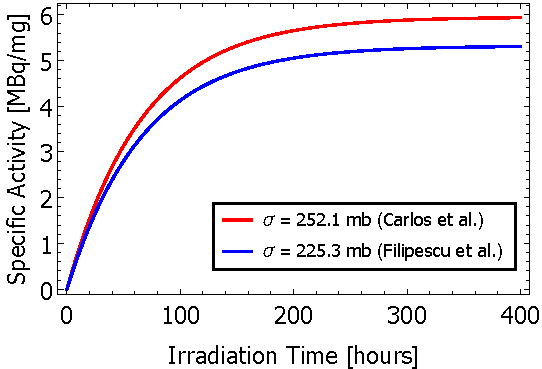
\includegraphics[width=0.6\textwidth]{Figures/DIANA_Inverse_Compton_Source_Design/154Sm_specific_activity.pdf}
\caption{Estimated specific activity of the produced $^{153}\mathrm{Sm}$ as a function of irradiation time using the collimated flux of the DIANA ICS source operating in a 0.5\% \textit{rms} bandwidth at the peak photoneutron reaction cross section, as measured by Carlos et al \cite{carlos1974giant} (red) and Filipescu et al \cite{filipescu2014photoneutron} (blue).}
\label{fig:153Sm_specific_activity}
\end{figure}

As shown in Fig.~\ref{fig:153Sm_specific_activity}, within around 10 days of irradiation the specific activity of the sample reaches a maximum of 66.92~\si{\mega\becquerel}/\si{\milli\gram} (Carlos et al \cite{carlos1974giant}) and 61.07~\si{\mega\becquerel}/\si{\milli\gram} (Filipescu et al \cite{filipescu2014photoneutron}). However, if there are irradiation time constraints, as is likely, the radioisotopic sample will not achieve the saturated specific activity. 

Typically, Quadramet is produced for clinical applications with a specific activity of 16--65~\si{\mega\becquerel}/\si{\micro\gram} \cite{ema2015quadramet}, a factor of $\sim$1000 below the current estimate for the photoneutron route. Therefore, photonuclear production of $^{153}\mathrm{Sm}$ is currently below viable commercial production standards because of the low reaction cross section, flux limitations of the DIANA ICS source and a lack of optimisation of this method. With optical cavities on the 100's~\si{\kilo\watt} scale becoming widely available \cite{eggl2016munich,liu2018optical}, the possibility of improving interaction dynamics using crab cavities \cite{variola2011luminosity,koshiba2018luminosity} and the increasing the average power frontier of ERLs, photonuclear production of radioisotopes could become plausible. There is also the additional possibility of increasing specific activity by targeting nuclear resonances for improved photoneutron reaction cross sections \cite{habs2011production}, though this hasn't been investigated within this work. However, proof-of-principle experiments involving photoneutron production of $^{153}\mathrm{Sm}$ could be conducted at the DIANA $\gamma$-ray ICS source, and optimisation of photonuclear production of radioisotopes is a possible topic for future work.      


\section{Summary}

\end{document}